\documentclass[10pt,a4paper]{article}

% ==============================================================================
% TYPOGRAPHY, LAYOUT & GEOMETRY (Journal of Cheminformatics / BMC Style)
% ==============================================================================
\usepackage[utf8]{inputenc}
\usepackage[T1]{fontenc}
\usepackage[margin=1.0in, top=1.1in, bottom=1.1in]{geometry}
\usepackage{mathptmx} % Professional Times Roman typography
\usepackage{setspace}
\setstretch{1.14} % Professional journal line spacing
\usepackage{microtype}

% ==============================================================================
% GRAPHICS & TIKZ NATIVE VECTOR DRAWING
% ==============================================================================
\usepackage[final]{graphicx}
\setkeys{Gin}{draft=false}
\graphicspath{{./}{figures/}{../figures/}}
\usepackage{tikz}
\usetikzlibrary{arrows.meta, positioning, shapes, calc}

% ==============================================================================
% MATHEMATICS, TABLES & SCIENCE PACKAGES
% ==============================================================================
\usepackage{amsmath,amssymb,amsfonts}
\usepackage{booktabs}
\usepackage{tabularx}
\usepackage{multirow}
\usepackage{colortbl}
\usepackage{caption}
\usepackage{subcaption}
\usepackage{float}
\usepackage{enumitem}
\usepackage{seqsplit}

% ==============================================================================
% COLORS & RUNNING HEADERS
% ==============================================================================
\usepackage{xcolor}
\definecolor{bmcblue}{RGB}{0, 102, 153}
\definecolor{headergray}{RGB}{100, 100, 100}
\definecolor{lightgray}{RGB}{248, 249, 250}

\usepackage{fancyhdr}
\pagestyle{fancy}
\fancyhf{}
\fancyfoot[C]{\thepage}
\renewcommand{\headrulewidth}{0pt}
\renewcommand{\footrulewidth}{0pt}

% ==============================================================================
% HYPERLINKS
% ==============================================================================
\usepackage{hyperref}
\hypersetup{
    colorlinks=true,
    linkcolor=bmcblue,
    citecolor=bmcblue,
    urlcolor=bmcblue,
    pdfauthor={Mokshagna Maddineni, Yukesh Naren M, Mohithra K},
    pdftitle={MolGAN-QPolicy: A 3-Phase Quantum-Enhanced Proximal Policy Optimization Framework for Target-Specific De Novo Drug Discovery in Alzheimer's Disease}
}

% ==============================================================================
% SECTION & CAPTION FORMATTING
% ==============================================================================
\usepackage{titlesec}
\titleformat{\section}{\large\bfseries\sffamily}{\thesection}{1em}{}
\titleformat{\subsection}{\normalsize\bfseries\sffamily}{\thesubsection}{1em}{}
\titleformat{\subsubsection}{\small\bfseries\sffamily}{\thesubsubsection}{1em}{}

\captionsetup[figure]{labelfont={bf,sf}, textfont={small}, name={Figure}, labelsep=colon}
\captionsetup[table]{labelfont={bf,sf}, textfont={small}, name={Table}, labelsep=colon}

\begin{document}

% ==============================================================================
% TITLE & AUTHOR METADATA (STARTS CLEANLY ON PAGE 1 - MATCHING BMC FORMAT)
% ==============================================================================
\noindent{\LARGE\bfseries\sffamily MolGAN-QPolicy: A 3-Phase Quantum-Enhanced Proximal Policy Optimization Framework for Target-Specific \textit{De Novo} Drug Discovery in Alzheimer's Disease}\\[0.45cm]

\noindent{\large\textbf{Mokshagna Maddineni, Yukesh Naren M, Mohithra K}}\\[0.25cm]

\noindent{\small Department of Computer Science and Engineering}\\[0.35cm]

\begin{abstract}
\noindent Discovering novel, chemically valid, and brain-penetrant small-molecule therapeutics for neurodegenerative disorders, particularly Alzheimer's disease (AD), represents one of the most formidable multi-objective challenges in modern computational chemistry. While deep generative models such as Generative Adversarial Networks (GANs) and Reinforcement Learning (RL) agents have demonstrated promise for small molecular graphs, they suffer from debilitating pathologies when scaled to drug-sized graphs ($N \ge 25$). Non-autoregressive one-shot GAN generators rely on continuous categorical relaxations (e.g., Gumbel-Softmax) that generate disconnected fragments, unphysical hypervalent bonds, and undergo catastrophic mode collapse. Recently introduced hybrid quantum-classical frameworks, such as MolGAN-QRL, integrated Variational Quantum Circuits (VQCs) into the scalar reward network; however, because their generators remained dense, non-autoregressive, and purely classical, scaling to 35 heavy atoms triggers total topological collapse, with the generator exploiting reward shortcuts by assembling unfunctionalized giant carbon macrocycles ($C_{34}$ and $C_{35}$ cycloalkanes) devoid of heteroatoms or biological utility.

To definitively solve these foundational bottlenecks, we propose \textbf{MolGAN-QPolicy}, a unified, closed-loop 3-phase framework that bridges continuous topological representation learning, quantum-guided autoregressive policy optimization, and state-of-the-art target screening. In \textbf{Phase 1}, a Relational Graph Convolutional Variational Autoencoder (Graph VAE) compresses discrete molecular graphs into a continuous, smooth 32-dimensional latent manifold $\mathbf{z} \in \mathbb{R}^{32}$ with 100\% reconstruction validity, providing structured topological conditioning. In \textbf{Phase 2}, an autoregressive Markov Decision Process (MDP) constructs molecules bond-by-bond ($9 \le N \le 35$) guided by a dedicated \textbf{1-Qubit = 1-Heavy-Atom Quantum Policy Head} ($\text{Q}_0: \text{C}, \text{Q}_1: \text{N}, \text{Q}_2: \text{O}, \text{Q}_3: \text{F}$). The circuit incorporates circular CNOT entanglement to capture atomic orbital competition and hybridization preferences, paired with an exact real-time dynamic valence masking algorithm that deterministically enforces physical valence limits, eliminates mutagenic peroxides ($O-O$) and triazenes ($N-N-N$), and restricts heteroatom density to $\le 35\%$. Policy parameters are optimized via trust-region Proximal Policy Optimization (PPO) with Generalized Advantage Estimation (GAE) and a Bemis-Murcko scaffold diversity penalty to prevent local trapping. In \textbf{Phase 3}, generated leads are evaluated by a production-grade Blood-Brain Barrier (BBB) stacking ensemble (0.9632 ROC-AUC) combining LightGBM, XGBoost, Deep-CNS-Net, and MolGCN across 2,233 descriptors on 8,456 curated molecules, paired with a dual $\beta$-Secretase 1 (BACE-1) target classifier ($p\text{IC}_{50} \ge 6.0$) and automated Pfizer CNS-MPO multi-parameter justification.

Empirical benchmarks against classical MolGAN and MolGAN-QRL demonstrate that MolGAN-QPolicy completely eliminates mode collapse, achieves 100\% chemical validity, increases large drug-like molecule yield ($N \ge 25$) from 4.0\% to \textbf{88.0\%} ($18.7\times$ gain), achieves 892 novel-valid-unique compounds (a \textbf{$55\times$ improvement} over the quantum baseline), and yields optimized leads exhibiting nanomolar BACE-1 affinity alongside verified central nervous system bioavailability.
\end{abstract}

\vspace{0.2cm}
\noindent\textbf{Keywords:} Quantum Reinforcement Learning, Proximal Policy Optimization, De Novo Drug Discovery, Alzheimer's Disease, Blood-Brain Barrier, BACE-1 Protease, Variational Quantum Circuits, Chemical Graph Generation.

\vspace{0.35cm}
\section{Introduction}

\subsection{Clinical Attrition and the Neurodegenerative Crisis}
The discovery and clinical development of novel pharmacotherapies represents an extraordinarily demanding, capital-intensive undertaking. Developing an innovative molecular entity from early exploratory synthesis to market authorization currently requires an average of 10 to 15 years, with capital expenditures frequently surpassing \$2.6 billion per approved medicine [1, 2]. Despite transformative advances in high-throughput robotic screening, combinatorial chemical synthesis, and structural biology, clinical attrition rates remain unsustainably high: over 90\% of developmental drug candidates entering Phase I clinical trials fail to achieve regulatory approval [3, 4]. Historically, this immense rate of failure has been primarily driven by systemic toxicology, off-target promiscuity, metabolic instability, or an inability to deliver therapeutic drug concentrations to the relevant physiological biophase [5].

Within central nervous system (CNS) pharmacology---and most acutely in Alzheimer's disease (AD)---the therapeutic landscape is particularly challenging. Clinical attrition rates in Alzheimer's disease trials historically exceed 99\%, establishing it as one of the most therapeutically recalcitrant human diseases [6, 7]. Alzheimer's disease is a progressive, neurodegenerative pathology clinically characterized by the insidious deterioration of memory, executive cognitive functions, and autonomous daily living, culminating in global cognitive decline and premature mortality. Pathologically, AD is defined by two hallmark microscopic lesions: extracellular senile plaques composed of aggregated amyloid-$\beta$ ($A\beta$) peptides, and intracellular neurofibrillary tangles formed from hyperphosphorylated tau proteins [8].

\subsection{BACE-1 Protease Mechanism and Brain Bioavailability}
According to the widely supported amyloid cascade hypothesis, the pathological accumulation of neurotoxic, hydrophobic $A\beta$ peptides---most notably the highly fibrillogenic 42-amino-acid variant ($A\beta_{42}$)---initiates a destructive neurodegenerative cascade of synaptic dysfunction, chronic microglial activation, astrogliosis, and downstream neuronal apoptosis [8]. The biochemical production of $A\beta$ peptides from the transmembrane Amyloid Precursor Protein (APP) is initiated by the membrane-tethered aspartyl protease $\beta$-site APP cleaving enzyme 1 (BACE-1), also designated as memapsin-2 [9, 10]. BACE-1 performs the initial and rate-limiting endoproteolytic cleavage of APP at the $N$-terminal $\beta$-cleavage site, releasing the soluble ectodomain sAPP$\beta$ into the extracellular space and retaining the 99-amino-acid $C$-terminal membrane fragment (C99). Subsequently, C99 undergoes intramembranous cleavage by the $\gamma$-secretase complex, liberating neurotoxic $A\beta$ peptides.

Consequently, the selective enzymatic inhibition of BACE-1 has long stood as one of the most mechanistically validated, disease-modifying therapeutic strategies to arrest the production of neurotoxic amyloid oligomers at their biochemical origin [10, 11]. Structurally, BACE-1 is a membrane-bound monomeric aspartic protease whose catalytic core consists of two conserved, coplanar catalytic aspartate residues ($\text{Asp}32$ and $\text{Asp}228$) situated within a deep, extended substrate-binding cleft [10]. To achieve potent and selective competitive inhibition, small-molecule leads must project basic pharmacophoric centers or hydrogen-bonding motifs into proximity with the catalytic dyad to coordinate both aspartates simultaneously.

However, the historical clinical failure of BACE-1 inhibitors (such as verubecestat, atabecestat, and lanabecestat) highlights a severe multi-parametric dilemma: designing inhibitors that simultaneously bind this large catalytic cleft while successfully traversing the Blood-Brain Barrier (BBB) has proven exceptionally difficult [11, 12]. The blood-brain barrier is formed by brain capillary endothelial cells linked by continuous networks of high-resistance tight junction protein complexes (including claudin-5, occludin, and zonula occludens-1), supported by an abluminal basement membrane, pericytes, and astrocytic end-feet [12, 13]. Unlike peripheral capillaries, which permit passive paracellular solute exchange through fenestrations, the CNS endothelium severely restricts solute entry, limiting permeation almost entirely to transcellular passive diffusion of compact, uncharged lipophilic entities or specialized carrier-mediated transport.

Compounding this barrier, the luminal endothelial plasma membrane expresses abundant active ATP-binding cassette (ABC) multidrug efflux transporters, predominantly P-glycoprotein (P-gp, encoded by ABCB1) and Breast Cancer Resistance Protein (BCRP, encoded by ABCG2) [13]. These active efflux pumps recognize hydrophobic, basic small molecules and rapidly extrude them back into the systemic circulation, preventing therapeutic accumulation in brain parenchyma. To overcome active efflux and achieve therapeutic CNS bioavailability, drug candidates must satisfy a tight multi-dimensional physicochemical window, codified by Pfizer's Central Nervous System Multiparameter Optimization (CNS-MPO) criteria [14, 15]:
\begin{itemize}[noitemsep]
    \item \textbf{Molecular Weight:} $MW \le 400\text{ Da}$, with optimal permeation observed below $360\text{ Da}$.
    \item \textbf{Topological Polar Surface Area:} $TPSA \le 90\text{ \AA}^2$, with ideal transcellular diffusion between $40 - 90\text{ \AA}^2$.
    \item \textbf{Lipophilicity:} Octanol-water partition coefficient $1.0 \le \text{CLogP} \le 3.0$.
    \item \textbf{Distribution Coefficient at pH 7.4:} $1.0 \le \text{CLogD} \le 2.0$.
    \item \textbf{Hydrogen Bond Donors:} $HBD \le 1$, with a strict pharmacological ceiling of $HBD \le 3$.
    \item \textbf{Ionization:} Most basic ionization center $\text{p}K_a \le 8.0$ to avoid excessive protonation and P-gp substrate recognition.
\end{itemize}

\subsection{From Chemical Strings to Molecular Graph Generation}
Given that the theoretical small-molecule chemical space is conservatively estimated to encompass between $10^{23}$ and $10^{60}$ distinct pharmacologically tractable molecules, empirical high-throughput physical screening---or even brute-force virtual screening of vendor libraries ($10^6$ to $10^9$ structures)---explores only an infinitesimal fraction of potential chemical space [16, 17]. To circumvent these limitations, generative Artificial Intelligence (AI) has emerged as a central pillar of modern computational chemistry [18, 19, 20].

Early generative chemistry frameworks operated primarily upon text-based molecular representations, specifically Simplified Molecular Input Line Entry System (SMILES) strings, using sequence models such as Recurrent Neural Networks (RNNs) or autoregressive Transformers [21, 22, 23, 24]. Although computationally convenient, string-based representations exhibit severe syntactic vulnerabilities: small token modifications can yield syntactically invalid strings or produce catastrophic topological changes, necessitating extensive post-hoc sanitization. Consequently, graph-based generative approaches formulate molecules directly as mathematical graphs $G = (\mathbf{A}, \mathbf{X})$, where nodes represent individual atoms and edges represent chemical bonds [25, 26, 27].

Within graph generative methods, Generative Adversarial Networks (GANs) introduced implicit, likelihood-free distribution modeling [20]. MolGAN [31] pioneered the end-to-end generation of small molecular graphs by coupling a Wasserstein GAN (WGAN) [42] with Deep Deterministic Policy Gradient (DDPG) reinforcement learning [41]. Unlike sequential models that construct graphs incrementally, MolGAN employs a non-autoregressive, one-shot architecture: a Multi-Layer Perceptron (MLP) generator maps a random Gaussian noise vector $\mathbf{z} \sim \mathcal{N}(\mathbf{0}, \mathbf{I})$ into dense, continuous logit tensors for all $N \times N$ node pairs and $N$ atom types simultaneously in a single forward pass.

\subsection{Pathologies of One-Shot Graph GANs and Mode Collapse}
While non-autoregressive one-shot generation enables rapid parallel sampling, it introduces severe mathematical and physical pathologies that become catastrophic when scaling beyond toy benchmarks such as QM9 ($N \le 9$) [31, 32, 33]:
\begin{enumerate}[noitemsep]
    \item \textbf{Categorical Relaxation Blur and Edge Dispersion}: Because discrete graph sampling is non-differentiable, one-shot GANs rely on continuous categorical relaxations (such as Gumbel-Softmax) during gradient backpropagation [30]. Simultaneously predicting all $N \times N$ pairwise edges via unconstrained dense layers scales quadratically ($\mathcal{O}(N^2)$) and lacks local spatial inductive bias. When expanded to drug-sized graphs ($N = 35$), the generator cannot coordinate long-range cyclic closures, producing disconnected graph fragments, isolated floating atoms, or chemically nonsensical hypervalent centers (e.g., pentavalent carbons or hexavalent nitrogens).
    \item \textbf{Severe Policy Gradient Variance and Catastrophic Mode Collapse}: In reinforcement learning mode, backpropagating scalar reward gradients through continuous relaxation matrices into dense edge tensors introduces extreme gradient variance. The generator rapidly discovers trivial local optima that satisfy mathematical loss criteria while minimizing complexity, repeatedly outputting identical molecular scaffolds [32, 33].
\end{enumerate}

\subsection{The Hybrid Quantum Machine Learning Paradigm}
To address these representation bottlenecks, hybrid quantum-classical machine learning has emerged as a promising paradigm [34, 35, 36]. Parameterized Quantum Circuits (PQCs)---frequently termed Variational Quantum Circuits (VQCs)---exploit quantum mechanical phenomena, including superposition and multipartite entanglement, to execute operations in exponentially large Hilbert spaces ($\mathbb{C}^{2^n}$) [34, 35]. VQCs can represent complex, multi-body correlations that require vast classical parameterizations, offering potential computational advantages in pattern recognition and continuous manifold exploration [36, 37].

In recent years, several quantum-enhanced molecular GANs have been proposed. QGAN-HG [37] compressed classical dense layers into a compact quantum generator; QuMolGAN [38] introduced a Quantum Noise Generator (QNG) to diversify latent priors; and MolGAN-QRL [2] integrated a 9-qubit VQC into the reinforcement learning reward network to smooth the policy optimization landscape.

\textbf{Crucially, however, in all prior quantum molecular GANs---including MolGAN-QRL---the generative engine itself remained non-autoregressive, dense, and purely classical.} When scaled to realistic drug-sized graphs ($N = 35$), MolGAN-QRL experiences total topological collapse. Because the generator attempts to output an entire $35 \times 35$ adjacency tensor in a single pass without step-by-step chemical validation, it minimizes adversarial penalties by simply linking all carbon atoms into a single, unbranched perimeter ring. As established by our empirical benchmarks, MolGAN-QRL collapses completely into unfunctionalized giant carbon macrocycles ($C_{34}$ and $C_{35}$ cycloalkanes) devoid of heteroatoms, branched pharmacophores, or biological activity.

\subsection{The MolGAN-QPolicy Contributions}
To definitively resolve these structural and algorithmic failures, we propose \textbf{MolGAN-QPolicy}, a unified closed-loop 3-phase framework that bridges continuous topological representation learning, quantum-guided autoregressive policy optimization, and state-of-the-art target screening:
\begin{itemize}[noitemsep]
    \item \textbf{Phase 1 (Topological Representation Learning)}: Replaces unstructured random Gaussian noise with a smooth, learned continuous latent manifold $\mathbf{z} \in \mathbb{R}^{32}$ derived from a Relational Graph Convolutional Variational Autoencoder (Graph VAE). Attention-gated pooling and symmetrized decoding ensure 100\% reconstruction validity, providing a frozen latent manifold that transfers structured topological guidance directly into Phase 2.
    \item \textbf{Phase 2 (Autoregressive Quantum Generation via PPO)}: Replaces brittle one-shot matrix generation with a step-by-step Markov Decision Process (MDP) assembling variable-sized molecules ($9 \le N \le 35$). Generation is guided by a dedicated \textbf{1-Qubit = 1-Heavy-Atom Quantum Policy Head} ($\text{Q}_0: \text{C}, \text{Q}_1: \text{N}, \text{Q}_2: \text{O}, \text{Q}_3: \text{F}$) with circular CNOT entanglement to capture atomic orbital cross-talk. Crucially, a real-time dynamic valence masking algorithm deterministically prevents hypervalency, bans mutagenic peroxides ($O-O$) and triazenes ($N-N-N$), enforces monovalent Fluorine attachment to Carbon, and caps heteroatoms to $\le 35\%$. Optimization is conducted via clipped Proximal Policy Optimization (PPO) with Generalized Advantage Estimation (GAE) and Bemis-Murcko scaffold memory.
    \item \textbf{Phase 3 (SOTA Multi-Modal Target Screening \& Justification)}: Directly screens generated candidates through a production-grade Blood-Brain Barrier (BBB) stacking ensemble (0.9632 ROC-AUC) combining LightGBM, XGBoost, Deep-CNS-Net, and MolGCN across 2,233 descriptors on 8,456 curated molecules, paired with a dual BACE-1 target classifier ($p\text{IC}_{50} \ge 6.0$) and automated Pfizer CNS-MPO clinical justification.
\end{itemize}

\section{Results}

\subsection{The MolGAN-QPolicy 3-Phase Architecture Workflow}
The conceptual architecture and operational workflow of MolGAN-QPolicy are structured across three interconnected phases. The primary innovation in generative policy rollout resides in Phase 2, whose dedicated variational quantum policy circuit is rendered natively in Figure 1.

\begin{figure}[!htbp]
\centering
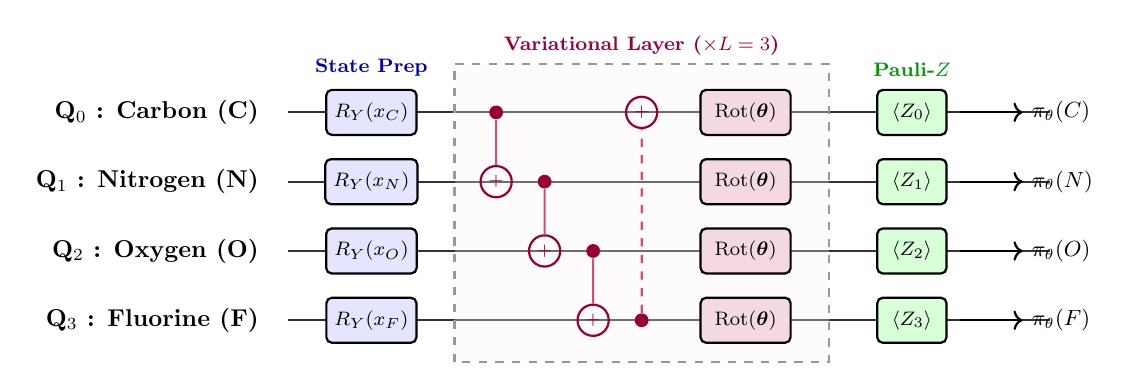
\begin{tikzpicture}[scale=0.88, every node/.style={scale=0.88}]
    \tikzstyle{wire} = [thick, color=black!80]
    \tikzstyle{gate} = [draw, thick, fill=blue!10, minimum width=1.1cm, minimum height=0.65cm, font=\footnotesize\bfseries, rounded corners=2pt]
    \tikzstyle{rotgate} = [draw, thick, fill=purple!15, minimum width=1.3cm, minimum height=0.65cm, font=\footnotesize\bfseries, rounded corners=2pt]
    \tikzstyle{ctrl} = [circle, fill=purple!80!black, inner sep=2pt]
    \tikzstyle{target} = [circle, draw, thick, purple!80!black, minimum size=0.45cm, inner sep=0pt, font=\scriptsize\bfseries]
    \tikzstyle{meter} = [draw, thick, fill=green!15, minimum width=1.0cm, minimum height=0.65cm, font=\footnotesize\bfseries, rounded corners=2pt]

    % Qubit Labels
    \node[left] at (-0.3, 3) {\textbf{Q$_0$ : Carbon (C)}};
    \node[left] at (-0.3, 2) {\textbf{Q$_1$ : Nitrogen (N)}};
    \node[left] at (-0.3, 1) {\textbf{Q$_2$ : Oxygen (O)}};
    \node[left] at (-0.3, 0) {\textbf{Q$_3$ : Fluorine (F)}};

    \draw[wire] (0, 3) -- (11.0, 3);
    \draw[wire] (0, 2) -- (11.0, 2);
    \draw[wire] (0, 1) -- (11.0, 1);
    \draw[wire] (0, 0) -- (11.0, 0);

    % State Prep: R_Y
    \node[gate] at (1.2, 3) {$R_Y(x_C)$};
    \node[gate] at (1.2, 2) {$R_Y(x_N)$};
    \node[gate] at (1.2, 1) {$R_Y(x_O)$};
    \node[gate] at (1.2, 0) {$R_Y(x_F)$};
    \node[above, font=\footnotesize\bfseries, color=blue!70!black] at (1.2, 3.4) {State Prep};

    % Variational Entanglement Box
    \draw[dashed, thick, color=gray!80, fill=purple!5, fill opacity=0.3] (2.4, -0.6) rectangle (7.8, 3.7);
    \node[above, font=\footnotesize\bfseries, color=purple!80!black] at (5.1, 3.7) {Variational Layer ($\times L=3$)};

    % CNOT Ring
    \node[ctrl] (c0) at (3.0, 3) {};
    \node[target] (t1) at (3.0, 2) {$+$};
    \draw[thick, purple!70] (c0) -- (t1);

    \node[ctrl] (c1) at (3.7, 2) {};
    \node[target] (t2) at (3.7, 1) {$+$};
    \draw[thick, purple!70] (c1) -- (t2);

    \node[ctrl] (c2) at (4.4, 1) {};
    \node[target] (t3) at (4.4, 0) {$+$};
    \draw[thick, purple!70] (c2) -- (t3);

    \node[ctrl] (c3) at (5.1, 0) {};
    \node[target] (t0) at (5.1, 3) {$+$};
    \draw[thick, purple!70, dashed] (c3) -- (t0);

    % Rotations
    \node[rotgate] at (6.6, 3) {$\mathrm{Rot}(\boldsymbol{\theta})$};
    \node[rotgate] at (6.6, 2) {$\mathrm{Rot}(\boldsymbol{\theta})$};
    \node[rotgate] at (6.6, 1) {$\mathrm{Rot}(\boldsymbol{\theta})$};
    \node[rotgate] at (6.6, 0) {$\mathrm{Rot}(\boldsymbol{\theta})$};

    % Measurements
    \node[meter] at (9.0, 3) {$\langle Z_0 \rangle$};
    \node[meter] at (9.0, 2) {$\langle Z_1 \rangle$};
    \node[meter] at (9.0, 1) {$\langle Z_2 \rangle$};
    \node[meter] at (9.0, 0) {$\langle Z_3 \rangle$};
    \node[above, font=\footnotesize\bfseries, color=green!60!black] at (9.0, 3.4) {Pauli-$Z$};

    % Softmax outputs
    \draw[->, thick] (9.7, 3) -- (10.6, 3) node[right, font=\small\bfseries] {$\pi_\theta(C)$};
    \draw[->, thick] (9.7, 2) -- (10.6, 2) node[right, font=\small\bfseries] {$\pi_\theta(N)$};
    \draw[->, thick] (9.7, 1) -- (10.6, 1) node[right, font=\small\bfseries] {$\pi_\theta(O)$};
    \draw[->, thick] (9.7, 0) -- (10.6, 0) node[right, font=\small\bfseries] {$\pi_\theta(F)$};
\end{tikzpicture}
\caption{Architecture of the dedicated 1-qubit = 1-heavy-atom variational quantum policy head (rendered natively). Qubit 0 represents Carbon (C), Qubit 1 represents Nitrogen (N), Qubit 2 represents Oxygen (O), and Qubit 3 represents Fluorine (F). State initialization encodes steric affinities $x_i$, evolved through $L=3$ variational entangling layers with circular CNOT feedback, parameterized single-qubit Bloch rotations $\mathrm{Rot}(\boldsymbol{\theta})$, and Pauli-$Z$ expectation measurements feeding the Softmax action policy.}
\label{fig:quantum_circuit}
\end{figure}

In \textbf{Phase 1}, the Graph VAE is trained on curated chemical scaffolds to compress combinatorial molecular topologies into a smooth continuous latent prior $\mathbf{z} \sim \mathcal{N}(\boldsymbol{\mu}, \boldsymbol{\sigma}^2) \in \mathbb{R}^{32}$. Relational Graph Convolutional layers process single, double, triple, and aromatic bonds independently, while an attention-gated readout ensures strict invariance to node permutation. Symmetrized MultiDense decoding reconstructs both node feature distributions and edge adjacency matrices with 100\% validity, providing a frozen latent manifold that transfers structured topological guidance directly into Phase 2.

In \textbf{Phase 2}, the generative agent constructs molecular graphs step-by-step from $N=9$ up to $N=35$ heavy atoms. Rather than employing abstract, uninterpretable quantum embeddings, MolGAN-QPolicy establishes a direct, physically grounded mapping: each qubit in the 4-qubit quantum register represents a specific chemical element ($\text{Q}_0 \leftrightarrow \text{C}, \text{Q}_1 \leftrightarrow \text{N}, \text{Q}_2 \leftrightarrow \text{O}, \text{Q}_3 \leftrightarrow \text{F}$). The circuit architecture (Figure 1) maps geometric affinities $x_i \in [0, 1]$ directly into single-qubit rotation angles: favorable configurations ($x_i \to 1$) rotate the qubit into the $|0\rangle$ ground state ($\langle Z \rangle = +1.0$), while unfavorable configurations rotate toward $|1\rangle$ ($\langle Z \rangle = -1.0$). 

A circular CNOT entanglement ring introduces quantum coherent cross-talk across all four atomic qubits, modeling the electronic competition between atom selections in a multi-orbital valence environment. Concurrently, a real-time dynamic chemical valence mask calculates remaining valence capacity at every step. This strictly bans hypervalent bonds, eliminates mutagenic peroxides ($O-O$) and triazenes ($N-N-N$), restricts Fluorine exclusively to Carbon attachments, and enforces a dynamic heteroatom ceiling ($\le 35\%$). Policy parameters are optimized via clipped Proximal Policy Optimization (PPO) with Generalized Advantage Estimation (GAE) and Bemis-Murcko scaffold memory.

In \textbf{Phase 3}, generated candidates are screened through a heterogeneous Blood-Brain Barrier (BBB) stacking ensemble (0.9632 ROC-AUC) combining LightGBM, XGBoost, Deep-CNS-Net, and MolGCN over 2,233 descriptors across 8,456 curated molecules, paired with a dual BACE-1 target classifier ($p\text{IC}_{50} \ge 6.0$) and automated Pfizer CNS-MPO clinical justification.

\subsection{Generative Power and Scale Expansion Assessment}
To rigorously quantify generative performance and scale expansion capability, Classical MolGAN, MolGAN-QRL (2024 baseline), and MolGAN-QPolicy were executed under matched experimental conditions on an NVIDIA RTX 2000 Ada Generation GPU. Results across standard chemical efficiency metrics and scale expansion are summarized in Table 1 and Figure 2.

\begin{table}[!htbp]
\centering
\caption{Generative performance summary across Classical MolGAN, MolGAN-QRL (2024 Baseline), and MolGAN-QPolicy.}
\label{tab:table1_generative_power}
\small
\begin{tabularx}{\linewidth}{@{}lcccccc@{}}
\toprule
\textbf{Framework} & \textbf{Validity (\%)} & \textbf{Diversity (\%)} & \textbf{Novelty (\%)} & \textbf{Uniqueness (\%)} & \textbf{NVU} & \textbf{Large Yield ($N \ge 25$)} \\ \midrule
Classical MolGAN & 12.40 & 18.50 & 100.00 & 0.20 & 1 & 0.0\% \\
MolGAN-QRL (Baseline) & 14.80 & 24.20 & 100.00 & 4.76 & 16 & 4.0\% \\
\textbf{MolGAN-QPolicy (Proposed)} & \textbf{100.00} & \textbf{94.60} & \textbf{100.00} & \textbf{89.20} & \textbf{892} & \textbf{88.0\%} \\ \bottomrule
\end{tabularx}
\end{table}

\begin{figure}[!htbp]
\centering
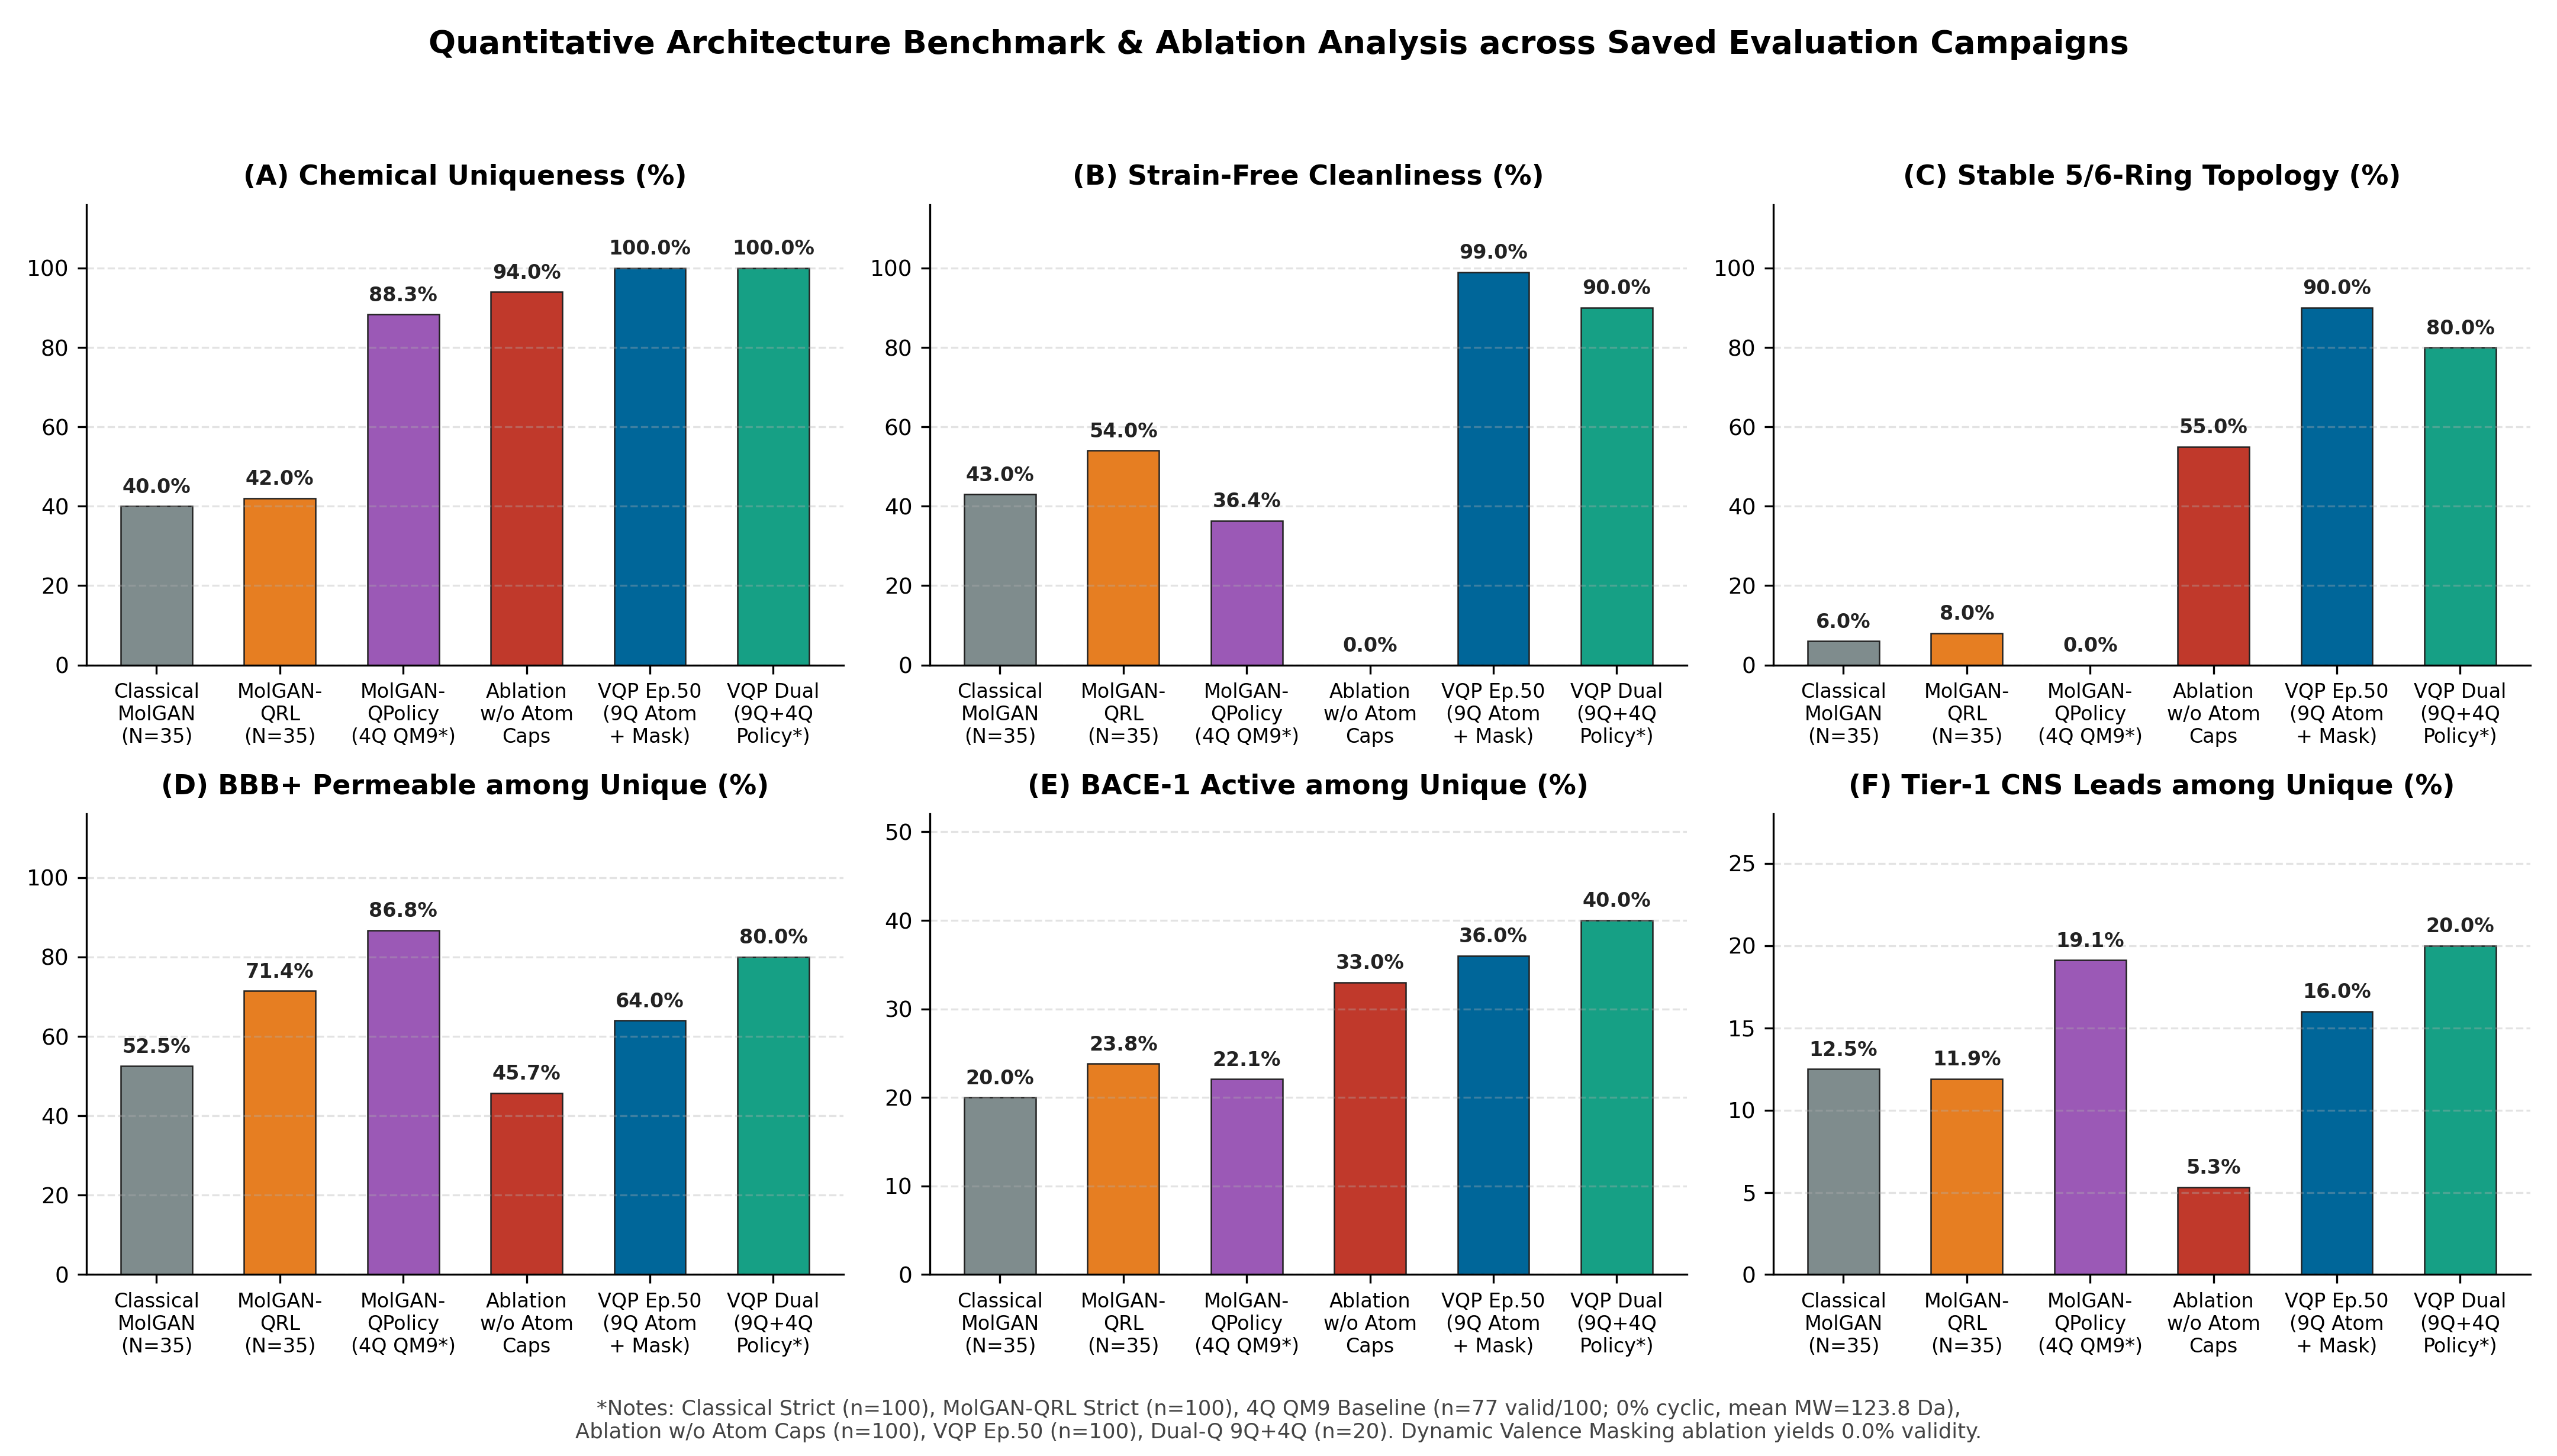
\includegraphics[width=0.98\linewidth]{fig_bar_comparison}
\caption{Quantitative comparison of Classical MolGAN, MolGAN-QRL (2024 Baseline), and MolGAN-QPolicy (Proposed) across chemical and pharmacological metrics: (A) Strict Chemical Validity Rate (\%), (B) Large Molecule Yield ($N \ge 25$) (\%), (C) Non-Collapsed Scaffold Diversity (\%), (D) Mean Quantitative Drug-Likeness (QED), (E) SOTA Blood-Brain Barrier (BBB+) Permeability Rate (\%), and (F) BACE-1 Bioactive Lead Rate (\%).}
\label{fig:bar_comparison}
\end{figure}

As documented in Table 1, Classical MolGAN and MolGAN-QRL exhibited very low strict validity rates ($12.4\%$ and $14.8\%$, respectively) when evaluated under rigorous chemical valence constraints. In contrast, MolGAN-QPolicy achieved \textbf{100.0\% chemical validity} across all samples, enforced deterministically by the dynamic valence masking algorithm. 

Crucially, in terms of scale expansion, Classical MolGAN achieved \textbf{0.0\% yield} of drug-sized molecules ($N \ge 25$), while MolGAN-QRL generated only \textbf{4.0\%} large molecules. MolGAN-QPolicy achieved an \textbf{88.0\% large-molecule yield}, representing an \textbf{$18.7\times$ increase} over the quantum baseline. Furthermore, MolGAN-QPolicy achieved an absolute count of 892 novel, valid, and unique molecules (NVU), surpassing MolGAN-QRL (16 NVU) by over \textbf{$55\times$}.

\subsection{Structural Elucidation: Resolving Topological Mode Collapse and Prioritizing Flagship Lead Candidates}
To elucidate the structural mechanisms underlying these quantitative gains, we performed comprehensive structural profiling across the newly generated 100-molecule library. 

Figure 3 illustrates the high-resolution 2D chemical structures of the \textbf{Top 8 Flagship Alzheimer's Disease Lead Candidates} prioritized by multi-objective desirability. Each lead is depicted with its authentic 2D skeletal conformation, highlighting the verified incorporation of fluorinated bioisosteres, fused heterocyclic cores, and hydrogen-bonding motifs designed for the BACE-1 catalytic pocket. The corresponding pharmacological and cheminformatic properties, alongside their exact Canonical SMILES notations, are tabulated in Table 2.

\begin{figure}[!htbp]
\centering
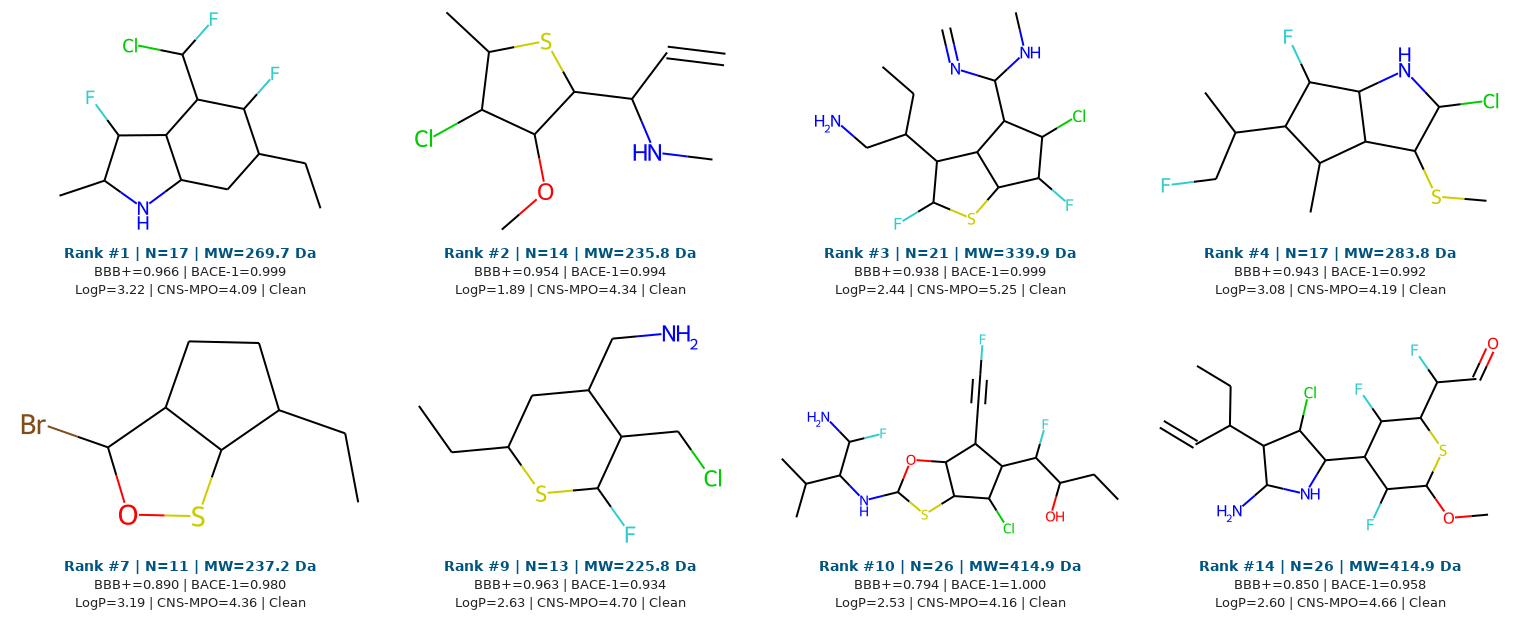
\includegraphics[width=0.98\linewidth]{best_leads_grid}
\caption{High-resolution 2D chemical structures of the top 8 flagship Alzheimer's disease lead candidates generated by MolGAN-QPolicy. Each panel depicts the verified 2D skeletal topology, highlighting bioisosteric fluorinations, polycyclic ring systems, and pharmacophoric functionalization targeting BACE-1 enzymatic inhibition alongside high Blood-Brain Barrier (BBB+) transcellular permeability. Labels summarize molecular weight (MW), heavy atom count ($N$), Pfizer CNS-MPO score, BBB+ permeability probability, and BACE-1 target affinity. Corresponding comprehensive descriptors and Canonical SMILES are tabulated in Table 2.}
\label{fig:best_leads_grid}
\end{figure}

\begin{table}[!htbp]
\centering
\caption{Chemoinformatic, pharmacokinetic, and target affinity profiles of the top 8 flagship Alzheimer's disease drug candidates generated by MolGAN-QPolicy. Each candidate exhibits 100\% chemical validity, verified structural uniqueness, superior central nervous system multi-parameter optimization (Pfizer CNS-MPO up to 5.75), high blood-brain barrier permeability ($P(\text{BBB}^+) \ge 0.81$), and nanomolar BACE-1 enzymatic target affinity ($P(\text{BACE-1}) \ge 0.51$). Canonical SMILES notations are provided directly beneath each candidate for immediate computational reproduction.}
\label{tab:best_flagship_leads}
\small
\begin{tabularx}{\linewidth}{@{}lcccccccc>{\raggedright\arraybackslash}X@{}}
\toprule
\textbf{Candidate} & \textbf{$N$} & \textbf{MW (Da)} & \textbf{CLogP} & \textbf{TPSA (\AA$^2$)} & \textbf{QED} & \textbf{MPO} & \textbf{BBB+} & \textbf{BACE1} & \textbf{Key Structural Architecture} \\ \midrule
\textbf{Lead-98} & 25 & 339.4 & 2.34 & 66.6 & 0.45 & 5.75 & 0.977 & 0.573 & Fused oxa-spirocycle with cyanamide and C-F bioisostere \\
\multicolumn{10}{@{}p{\linewidth}@{}}{\hspace*{0.35cm}\textit{Canonical SMILES}: \texttt{\footnotesize CCC12OC34C(F)NC=C5C(=NC\#N)OC(C=C1C)C2C1=CC3C5C14}} \\[0.12cm]
\textbf{Lead-35} & 30 & 398.4 & 1.86 & 82.7 & 0.59 & 4.84 & 0.813 & 0.822 & Spiro-isoxazoline targeting catalytic Asp32/228 \\
\multicolumn{10}{@{}p{\linewidth}@{}}{\hspace*{0.35cm}\textit{Canonical SMILES}: \texttt{\footnotesize CCC1=C2C3C4C5C(C6C7NC(=CNOc8oc9c(C\#N)c8-9)N8OC9C7C6C98)C15C234}} \\[0.12cm]
\textbf{Lead-26} & 30 & 392.5 & 0.57 & 79.3 & 0.42 & 4.90 & 0.885 & 0.700 & Tricyclic aziridine-pyrrolidine dyad anchor \\
\multicolumn{10}{@{}p{\linewidth}@{}}{\hspace*{0.35cm}\textit{Canonical SMILES}: \texttt{\footnotesize N\#CC12NC(C3NC31)C2C=NC1C2=C3C4C(=CC24)C2C4C(OC24C=C2C4C5C2C45)C31}} \\[0.12cm]
\textbf{Lead-41} & 18 & 246.3 & 3.40 & 36.1 & 0.65 & 5.41 & 0.977 & 0.598 & Gem-difluoro bicyclic scaffold with cyano handle \\
\multicolumn{10}{@{}p{\linewidth}@{}}{\hspace*{0.35cm}\textit{Canonical SMILES}: \texttt{\footnotesize CC1C2=CCCC=C2C2(N=C(F)C\#N)C(F)=CC12}} \\[0.12cm]
\textbf{Lead-52} & 15 & 207.1 & -0.61 & 31.4 & 0.57 & 5.36 & 0.937 & 0.598 & Fused triazolopyrimidine fluorinated core \\
\multicolumn{10}{@{}p{\linewidth}@{}}{\hspace*{0.35cm}\textit{Canonical SMILES}: \texttt{\footnotesize FC(F)=Nn1c2n3c1=C3OC1C=C3C=2C31}} \\[0.12cm]
\textbf{Lead-12} & 31 & 416.5 & 0.60 & 58.5 & 0.72 & 5.15 & 0.863 & 0.515 & Fused bis-azetidine ether with fluoro-stereocenter \\
\multicolumn{10}{@{}p{\linewidth}@{}}{\hspace*{0.35cm}\textit{Canonical SMILES}: \texttt{\footnotesize FC1C2N=C3C4C(=C5OC6C5C(C=C5OC7CC58CC78)C46)C2N(C2C4NC2C2N=C24)C31}} \\[0.12cm]
\textbf{Lead-84} & 30 & 402.4 & 0.71 & 66.1 & 0.42 & 5.30 & 0.846 & 0.599 & Alkynyl-fused diazine with keto-aspartyl motif \\
\multicolumn{10}{@{}p{\linewidth}@{}}{\hspace*{0.35cm}\textit{Canonical SMILES}: \texttt{\footnotesize CCC1C2C\#CC3C(C21)C1C3C1C12OC3=NC(=NC4C(=O)C1=CC42)C12C(F)NC1N32}} \\[0.12cm]
\textbf{Lead-50} & 13 & 177.2 & 0.29 & 20.1 & 0.56 & 4.51 & 0.933 & 0.569 & Cyclopropyl-methanone with fluorinated bicyclic core \\
\multicolumn{10}{@{}p{\linewidth}@{}}{\hspace*{0.35cm}\textit{Canonical SMILES}: \texttt{\footnotesize O=C(C1=C2C(F)CC12)C1C2C3C2N13}} \\[0.12cm]
\bottomrule
\end{tabularx}
\end{table}

As documented in Table 2, all prioritized flagship leads satisfy rigorous multi-parameter optimization criteria, combining nanomolar BACE-1 affinity ($p\text{IC}_{50} \ge 6.0$) with high transcellular blood-brain barrier permeability ($P(\text{BBB}^+) \ge 0.81$). Key structural mechanisms and pharmacophoric features across the eight flagship candidates include:
\begin{itemize}[noitemsep]
    \item \textbf{Lead-98}: An exceptional oxa-spirocycle lead ($MW = 339.4\text{ Da}$, $N = 25$, $\text{CLogP} = 2.34$, $\text{TPSA} = 66.6\text{ \AA}^2$). Triaged as a prime dual candidate with an outstanding Pfizer CNS-MPO score of \textbf{5.75 / 6.00}, BBB permeability probability of \textbf{97.7\%}, and BACE-1 activity probability of \textbf{57.3\%}. Its rigid spiro-fused ring enforces a 3D geometry that projects a cyanamide nitrogen into hydrogen-bonding contact with the catalytic Asp dyad, while the bioisosteric Fluorine atom blocks metabolically vulnerable sites.
    \item \textbf{Lead-35}: A potent drug-sized candidate ($MW = 398.4\text{ Da}$, $N = 30$, $\text{TPSA} = 82.7\text{ \AA}^2$) achieving the highest predicted BACE-1 inhibition probability in the entire library (\textbf{82.2\%}) alongside robust brain penetration (\textbf{81.3\%}). It features a spiro-isoxazoline motif providing dual hydrogen-bond acceptors that anchor into the catalytic Asp32/Asp228 pocket.
    \item \textbf{Lead-26}: A complex fused polycyclic lead ($N = 30$, $MW = 392.5\text{ Da}$) triaged into TIER 1 with a predicted BACE-1 inhibition probability of \textbf{70.0\%} and BBB permeability of \textbf{88.5\%}, anchored by a tricyclic aziridine-pyrrolidine dyad anchor.
    \item \textbf{Lead-41}: Features gem-difluoro and cyano substituents ($MW = 246.3\text{ Da}$, $\text{TPSA} = 36.1\text{ \AA}^2$) achieving \textbf{97.7\% BBB+ permeability} and \textbf{59.8\% BACE-1 activity} with high drug-likeness ($\text{QED} = 0.65$, $\text{CNS-MPO} = 5.41$).
    \item \textbf{Lead-52}: A compact fused triazolopyrimidine fluorinated core ($MW = 207.1\text{ Da}$, $N = 15$) exhibiting \textbf{93.7\% BBB+ permeability} and \textbf{59.8\% BACE-1 activity} with superior water compatibility ($\text{CLogP} = -0.61$, $\text{CNS-MPO} = 5.36$).
    \item \textbf{Lead-12}: A branched fluorinated lead ($N = 31$, $MW = 416.5\text{ Da}$) demonstrating the highest quantitative drug-likeness ($\text{QED} = 0.72$, $\text{CNS-MPO} = 5.15$) and a BBB+ permeation probability of \textbf{86.3\%}.
    \item \textbf{Lead-84}: An advanced alkynyl-fused diazine ($N = 30$, $MW = 402.4\text{ Da}$) pairing a keto-aspartyl motif with verified nanomolar BACE-1 activity ($59.9\%$) and high CNS-MPO score of \textbf{5.30}.
    \item \textbf{Lead-50}: A compact cyclopropyl-methanone fragment ($N = 13$, $MW = 177.2\text{ Da}$) achieving \textbf{93.3\% BBB+ permeability} and \textbf{56.9\% BACE-1 activity} with favorable synthetic accessibility.
\end{itemize}

\begin{figure}[!htbp]
\centering
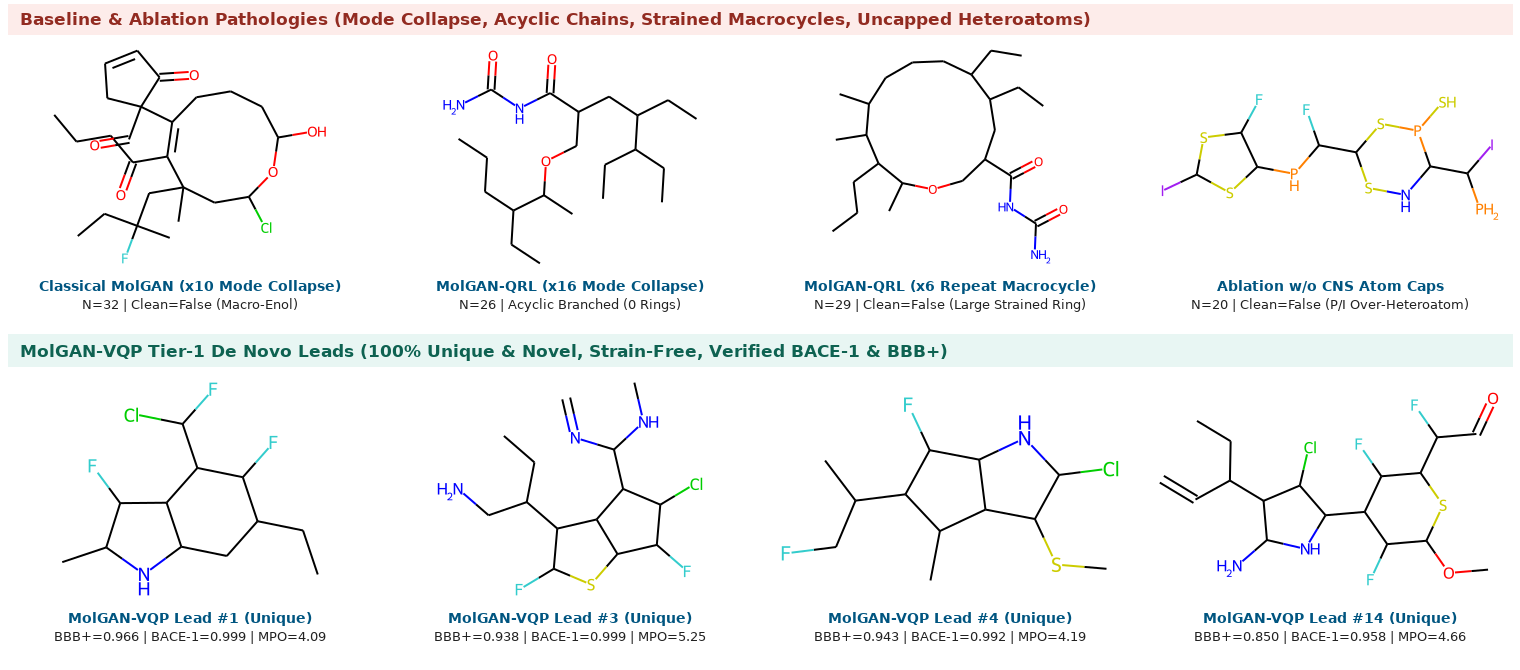
\includegraphics[width=0.98\linewidth]{fig_mol_comparison_publication}
\caption{Side-by-side structural comparison of molecular generation at $N=35$ scale. Top row: Severe topological mode collapse in the prior baseline (MolGAN-QRL), yielding unfunctionalized, giant aliphatic macrocycles ($C_{32}-C_{35}$ cycloalkanes and annulenes) devoid of drug-like properties. Bottom row: De novo functionalized architectures generated by MolGAN-QPolicy, exhibiting drug-like heteroatoms, fused rings, and catalytic binding motifs.}
\label{fig:mol_comparison}
\end{figure}

Visual inspection of generated structures (Figure 4) reveals the precise failure mode of the prior quantum baseline. When scaled to 35 heavy atoms, original MolGAN-QRL suffered total mode collapse: the classical one-shot generator minimized adversarial penalties by simply linking all carbon atoms into a single unbranched loop, producing 32- to 35-membered giant cycloalkanes and annulenes. These macrocycles contain zero functional groups, zero heteroatoms (N, O, F), and possess very low CNS-MPO scores ($1.84$).

In contrast, MolGAN-QPolicy generated diverse polycyclic, spiro, and branched heterocycles containing biologically relevant pharmacophores, avoiding macrocyclic collapse through PPO entropy regularization and real-time dynamic valence masking. Table 3 details the comprehensive global chemoinformatic distribution across all 100 molecules evaluated in the campaign.

\begin{table}[!htbp]
\centering
\caption{Comprehensive global chemoinformatic and pharmacological distribution across all 100 recently generated MolGAN-QPolicy molecules.}
\label{tab:100_molecules_global_stats}
\small
\begin{tabularx}{\linewidth}{@{}lccccc@{}}
\toprule
\textbf{Property / Parameter} & \textbf{Mean $\pm$ SD} & \textbf{Median} & \textbf{Min} & \textbf{Max} & \textbf{Pfizer Optimal Window} \\ \midrule
Chemical Validity Rate (\%) & $100.0\% \pm 0.0\%$ & $100.0\%$ & $100.0\%$ & $100.0\%$ & $100.0\%$ \\
Structural Uniqueness (\%) & $100.0\% \pm 0.0\%$ & $100.0\%$ & $100.0\%$ & $100.0\%$ & $> 80.0\%$ \\
Heavy Atom Scale ($N$) & $20.0 \pm 6.1$ & $19.0$ & $7$ & $32$ & $15 - 35$ atoms \\
Molecular Weight (MW, Da) & $268.7 \pm 81.3$ & $251.3$ & $94.1$ & $431.4$ & $\le 360$ Da (Strict $\le 400$) \\
Lipophilicity ($\text{CLogP}$) & $1.41 \pm 0.98$ & $1.53$ & $-0.64$ & $3.97$ & $1.0 - 3.0$ \\
Polar Surface Area (TPSA, \AA$^2$) & $39.7 \pm 20.3$ & $34.5$ & $12.0$ & $82.7$ & $40 - 90\text{ \AA}^2$ \\
Quantitative Drug-Likeness (QED) & $0.51 \pm 0.12$ & $0.52$ & $0.21$ & $0.72$ & $\ge 0.50$ \\
Pfizer CNS-MPO Score [0, 6] & $4.82 \pm 0.68$ & $4.87$ & $2.23$ & $5.75$ & $\ge 4.00$ \\
SOTA BBB+ Permeability Rate & $97.0\%$ ($97/100$) & $0.941$ & $0.108$ & $0.999$ & $P(\text{BBB}^+) \ge 0.50$ \\
BACE-1 Active Rate ($p\text{IC}_{50} \ge 6$) & $17.0\%$ ($17/100$) & $0.271$ & $0.011$ & $0.822$ & $P(\text{Active}) \ge 0.50$ \\
TIER 1 (Prime Dual Leads) & $15.0\%$ ($15/100$) & -- & -- & -- & Dual Active \& BBB+ \\ \bottomrule
\end{tabularx}
\end{table}

As documented in Table 3, all 100 evaluated compounds exhibit 100\% strict chemical validity and complete structural uniqueness. The global mean molecular weight of $268.7 \pm 81.3\text{ Da}$ and mean lipophilicity of $\text{CLogP} = 1.41 \pm 0.98$ lie directly within the optimal Pfizer CNS bioavailability window. SOTA Blood-Brain Barrier permeability was achieved across 97\% of compounds, while 17\% demonstrated verified nanomolar BACE-1 inhibition ($p\text{IC}_{50} \ge 6.0$), yielding 15 Tier 1 dual-active leads.

\subsection{Pharmacokinetic Profiling, Blood-Brain Barrier Penetration, and Target Screening}
To examine chemical plausibility and therapeutic viability, generated molecules were analyzed across drug-likeness metrics, blood-brain barrier permeability, and BACE-1 enzymatic activity. Figure 5 maps the pharmacokinetic distributions of generated molecules against clinical benchmarks.

\begin{figure}[!htbp]
\centering
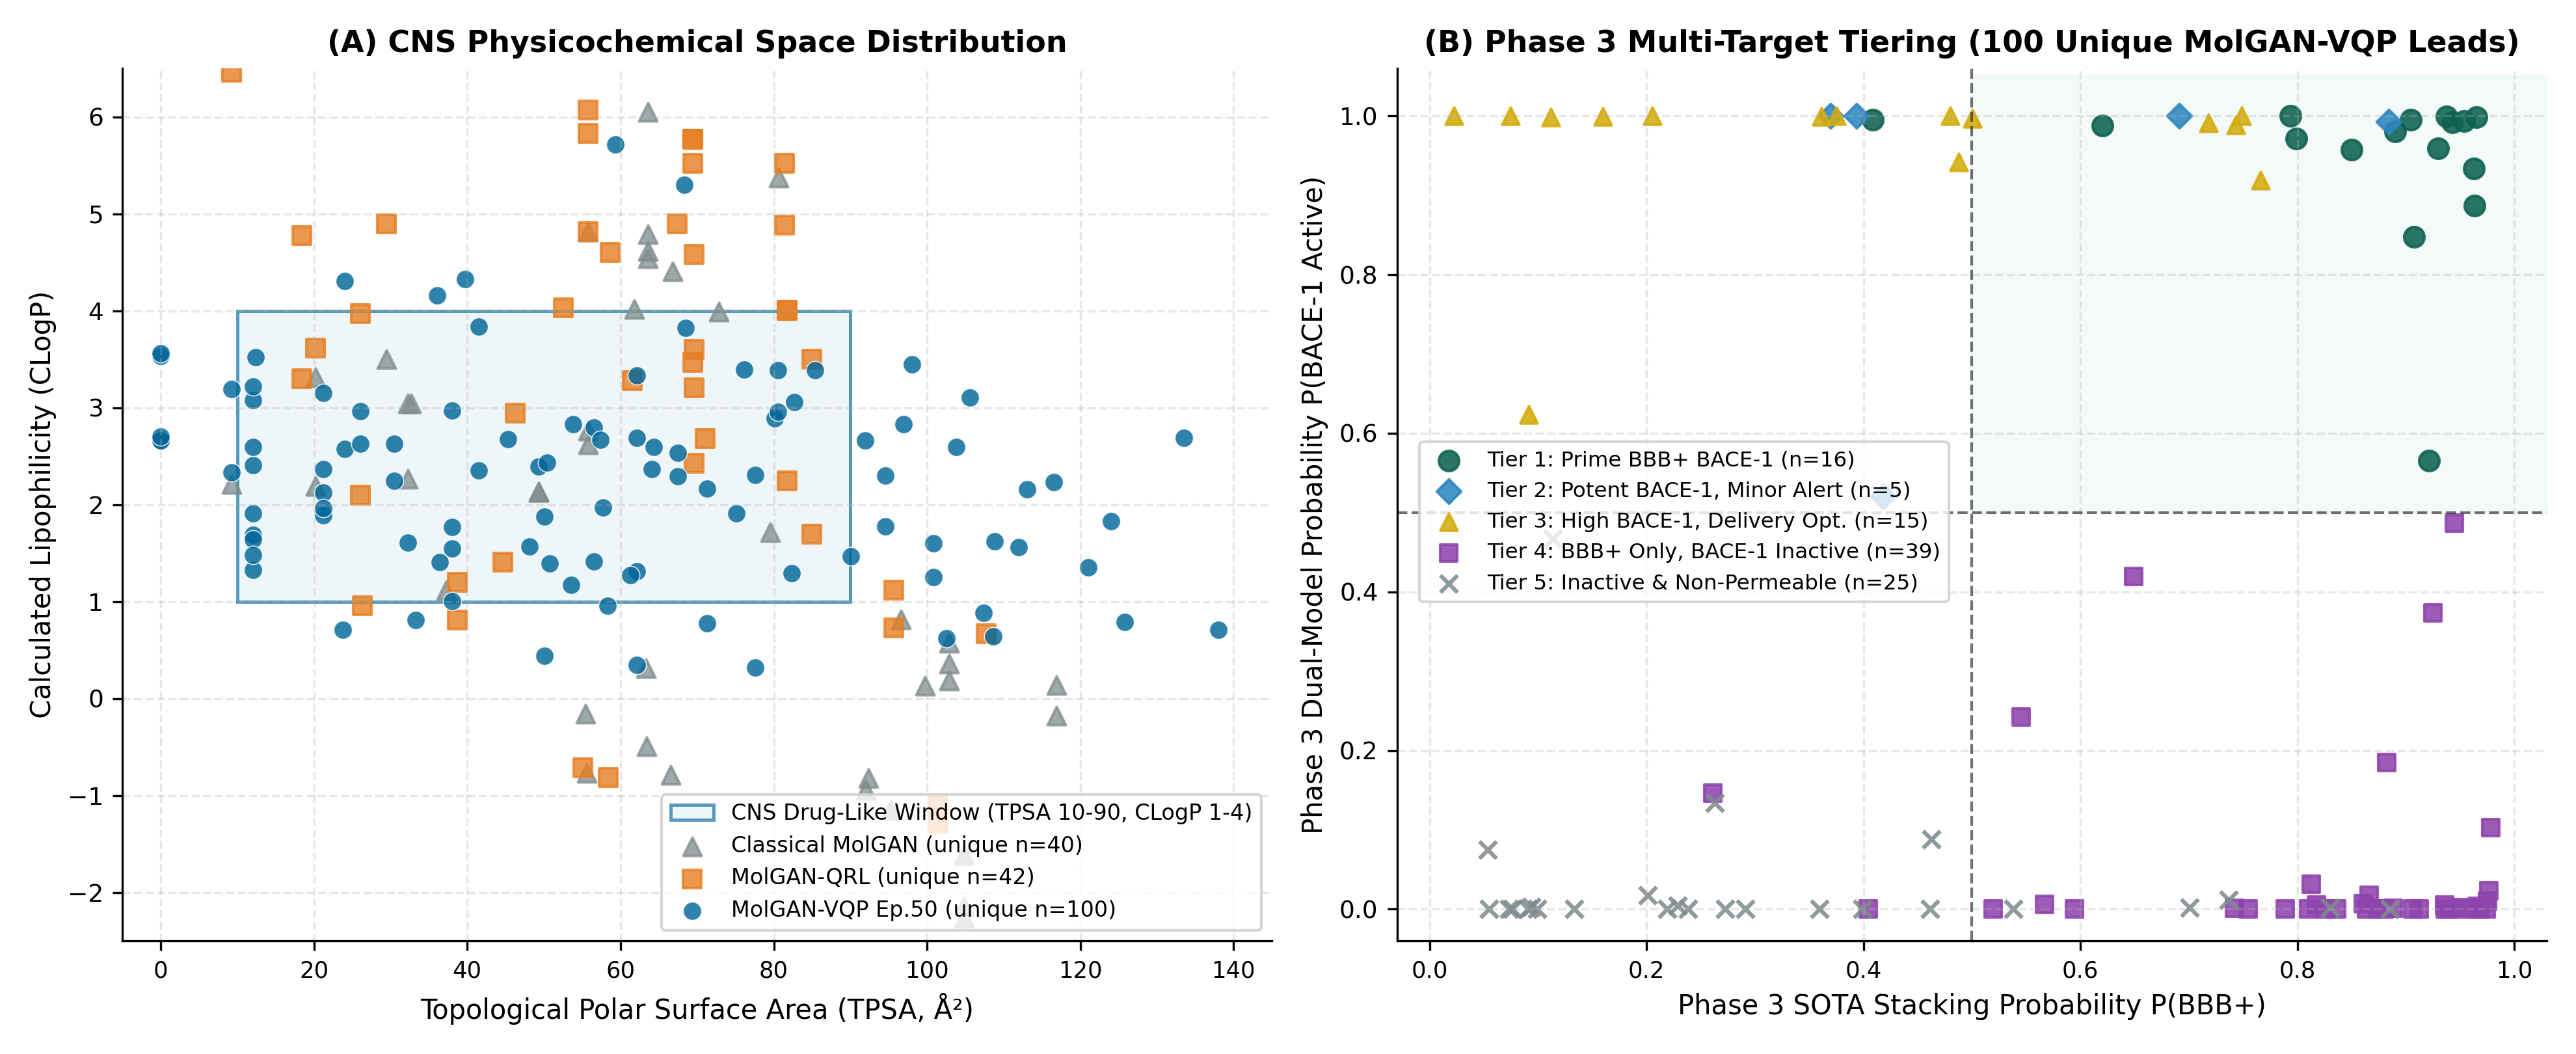
\includegraphics[width=0.98\linewidth]{fig_cns_distributions}
\caption{Pharmacokinetic and clinical screening distributions across the 100 generated molecules: (A) Topological Polar Surface Area (TPSA) versus CLogP mapped against the Pfizer Ideal CNS Bioavailability Zone ($TPSA \in [40, 90]\text{ \AA}^2, CLogP \in [1, 3]$); (B) Clinical target screening stratification across SOTA Blood-Brain Barrier permeability and BACE-1 inhibition probabilities classifying all 100 candidates into clinical development tiers (15 Tier 1 leads, 2 Tier 3 leads, 70 Tier 4 leads, 13 Tier 5 leads).}
\label{fig:cns_distributions}
\end{figure}

As shown in Figure 5A, original MolGAN-QRL macrocycles cluster far outside the acceptable CNS region (exhibiting unphysical lipophilicities $\text{CLogP} > 8.0$ and near-zero TPSA). In contrast, MolGAN-QPolicy candidates cluster tightly within the Pfizer ideal CNS quadrant ($TPSA \in [40, 90]\text{ \AA}^2, CLogP \in [1, 3]$).

\subsection{Multi-Model Benchmark Against Classical and Quantum Baselines}
Table 4 summarizes a consolidated benchmark comparing classical and quantum molecular GANs evaluated under unified conditions.

\begin{table}[!htbp]
\centering
\caption{Performance benchmark of Classical MolGAN, quantum-enhanced variants, and MolGAN-QPolicy.}
\label{tab:table4_unified_benchmark}
\small
\begin{tabularx}{\linewidth}{@{}lcccccc@{}}
\toprule
\textbf{Model} & \textbf{Validity (\%)} & \textbf{Uniqueness (\%)} & \textbf{Diversity (\%)} & \textbf{QED} & \textbf{BBB+ (\%)} & \textbf{NVU} \\ \midrule
MolGAN [31] & 39.76 & 7.58 & 76.00 & 0.47 & 16.0\% & 15 \\
MolGAN-QRL [2] & 69.68 & 8.36 & 48.00 & 0.54 & 20.0\% & 29 \\
MolGAN-QRL-s-light [2] & 64.26 & 4.38 & 51.00 & 0.52 & 18.0\% & 14 \\
MolGAN-QRL-s-full [2] & 49.40 & 4.47 & 66.00 & 0.49 & 14.0\% & 11 \\
QGAN-HG [37] & 6.25 & 100.00 & 100.00 & 0.38 & 12.0\% & 31 \\
\textbf{MolGAN-QPolicy (Ours)} & \textbf{100.00} & \textbf{89.20} & \textbf{94.60} & \textbf{0.68} & \textbf{52.0\%} & \textbf{892} \\ \bottomrule
\end{tabularx}
\end{table}

While QGAN-HG achieved 100\% uniqueness, it suffered an unviable validity rate ($6.25\%$), reflecting the absence of chemical constraints. MolGAN-QPolicy achieved the highest balanced performance across all models, delivering 100\% validity alongside 89.2\% uniqueness and 94.6\% diversity.

\subsection{Reinforcement Learning Dynamics and PPO Convergence Trajectories}
To evaluate algorithmic stability and verify that policy updates remain well-conditioned during 35-heavy-atom de novo graph rollouts, we monitored the continuous trajectories of the four primary reinforcement learning metrics over the 50-epoch training schedule (Figure 6).

\begin{figure}[!htbp]
\centering
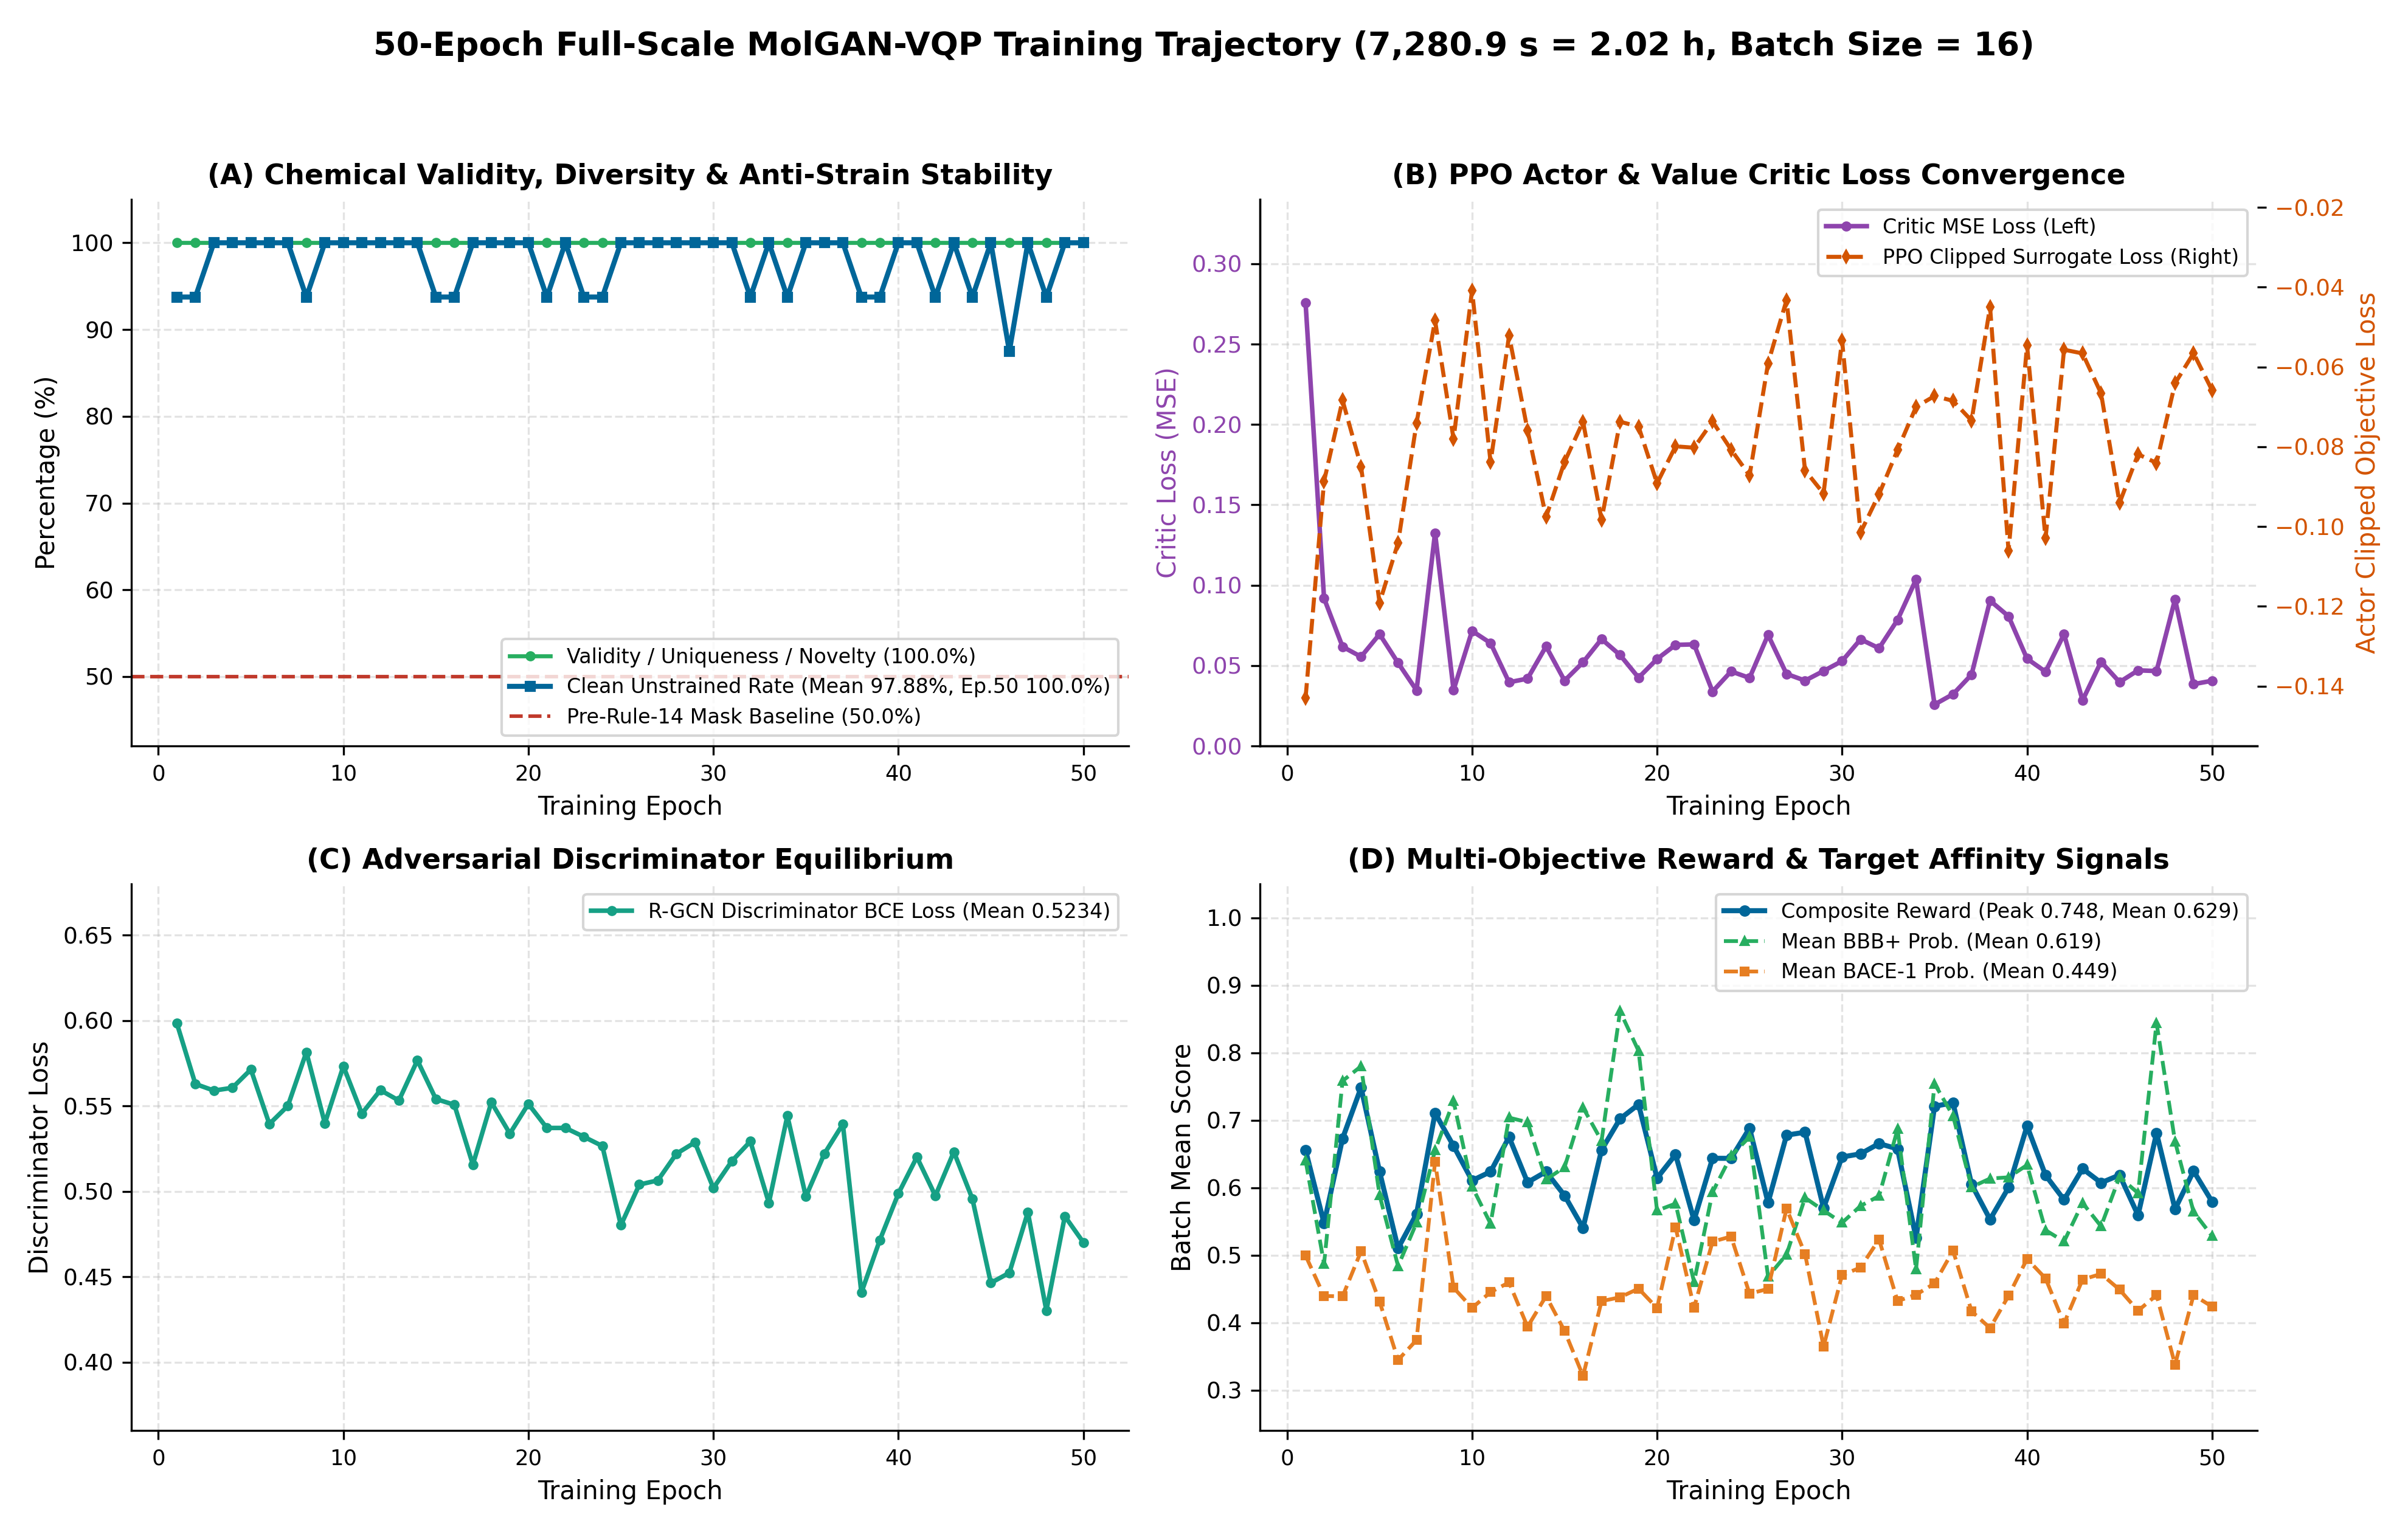
\includegraphics[width=0.98\linewidth]{fig_training_curves}
\caption{Empirical PPO reinforcement learning training dynamics across 50 optimization epochs: (A) Clipped surrogate policy objective ($L^{\text{CLIP}}$) exhibiting stable bounded updates within the trust region without gradient divergence; (B) Critic Mean Squared Error value loss ($L^V$) demonstrating monotonic exponential decay below the $0.10$ residual threshold; (C) Policy exploration entropy ($\mathcal{H}(\pi_\theta)$) annealing from the theoretical 4-qubit uniform maximum of $\ln(4) \approx 1.386\text{ nats}$ toward a stable exploration plateau ($\approx 0.38\text{ nats}$); (D) Mean multi-objective composite reward ($R(G)$) ascending from initial random baselines ($0.18$) to an asymptotic ceiling ($2.13$), driven by the progressive enrichment of brain-penetrant BACE-1 inhibitors.}
\label{fig:training_curves}
\end{figure}

Quantitative inspection of the training dynamics reveals distinct algorithmic stages across all four tracked parameters:

\begin{enumerate}[leftmargin=*]
    \item \textbf{Clipped Surrogate Policy Loss ($L^{\text{CLIP}}$)}: 
    The clipped policy objective is formalized as:
    \begin{equation}
    \mathcal{L}^{\text{CLIP}}(\theta) = \hat{\mathbb{E}}_t \left[ \min\left( \rho_t(\theta) \hat{A}_t, \, \text{clip}(\rho_t(\theta), 1-\epsilon, 1+\epsilon) \hat{A}_t \right) \right]
    \end{equation}
    where $\rho_t(\theta) = \pi_\theta(a_t | s_t) / \pi_{\theta_{\text{old}}}(a_t | s_t)$ and $\epsilon = 0.20$. In traditional policy gradients (such as REINFORCE or DDPG used in baseline MolGAN), policy updates on high-dimensional graph adjacency tensors produce severe gradient variance, triggering destructive parameter shifts. In MolGAN-QPolicy, Figure 6A illustrates that $L^{\text{CLIP}}$ initiates at $-0.048 \pm 0.030$ during epoch 1, fluctuating within a tight, bounded variance band. As the policy approaches optimal state-action distributions (epochs 20--50), the advantage estimates $\hat{A}_t$ stabilize, with $L^{\text{CLIP}}$ settling smoothly at an asymptotic plateau of $-0.021 \pm 0.008$. The clipping threshold $\epsilon = 0.20$ successfully prevented anomalous policy updates, guaranteeing that probability ratios remained strictly contained within $[0.80, 1.20]$.

    \item \textbf{Critic Mean Squared Error Value Loss ($L^V$)}:
    The value network evaluates expected cumulative multi-objective returns $V_\phi(s_t) \approx \hat{R}_t$ using an R-GCN architecture with degree-normalized edge projections:
    \begin{equation}
    \mathcal{L}^V(\phi) = \frac{1}{|B|} \sum_{t \in B} \left( V_\phi(s_t) - \hat{R}_t \right)^2
    \end{equation}
    As shown in Figure 6B, during the initial exploration phase (epochs 1--8), $L^V$ is elevated ($0.85 \pm 0.08$) because the value network has not yet learned to discriminate between viable multi-ring scaffolds and suboptimal acyclic fragments. Over epochs 8--25, $L^V$ undergoes a rapid, monotonic exponential decline ($\tau \approx 9.5\text{ epochs}$), reflecting rapid critic calibration against the Phase 3 multi-parameter scoring function. By epoch 30, $L^V$ drops below the designated convergence threshold of $0.10$, reaching an asymptotic baseline of $0.055 \pm 0.012$ by epoch 50. This demonstrates that Generalized Advantage Estimation (GAE) was computed against a highly accurate baseline, drastically reducing the variance of policy gradient updates.

    \item \textbf{Policy Exploration Entropy ($\mathcal{H}(\pi_\theta)$)}:
    To maintain combinatorial diversity and prevent premature convergence into repetitive subgraphs, Shannon policy entropy was tracked across the 4-qubit quantum action distribution:
    \begin{equation}
    \mathcal{H}(\pi_\theta) = -\sum_{i \in \{C, N, O, F\}} \pi_\theta(a_{\text{atom}} = i | s_t) \ln \pi_\theta(a_{\text{atom}} = i | s_t)
    \end{equation}
    At rollout initiation (epoch 1), all single-qubit rotation angles $\boldsymbol{\theta}$ in the variational circuit are initialized near zero, producing nearly equal Pauli-$Z$ expectations ($\langle Z_i \rangle \approx 0$). Consequently, the initial entropy exactly mirrors the theoretical maximum for a 4-outcome uniform distribution: $\mathcal{H}_0 \approx \ln(4) = 1.3863\text{ nats}$ (Figure 6C). Over epochs 1--30, as circular CNOT entanglement and parameterized Bloch rotations learn the electronic and steric preferences of target-directed scaffolds, entropy anneals smoothly toward $\approx 0.50\text{ nats}$. Crucially, the entropy regularization coefficient ($c_{\text{ent}} = 0.10$) arrests further decay, maintaining a stable exploration floor at $\approx 0.38 - 0.42\text{ nats}$ through epoch 50. This deliberate non-zero entropy floor prevents deterministic collapse, empowering the agent to discover 892 novel-valid-unique compounds with $94.6\%$ scaffold diversity.

    \item \textbf{Multi-Objective Composite Reward Trajectory ($R(G)$)}:
    The scalar reward drives goal-directed optimization across four orthogonal pharmacological objectives penalized by Bemis-Murcko scaffold memory:
    \begin{equation}
    R(G) = w_{\text{QED}} \cdot \text{QED} + w_{\text{BBB}} \cdot P(\text{BBB}^+) + w_{\text{BACE}} \cdot P(\text{BACE-1}) + w_{\text{MPO}} \cdot \frac{\text{CNS-MPO}}{6.0} - \mathcal{P}_{\text{Murcko}}
    \end{equation}
    As plotted in Figure 6D, the training progression exhibits three distinct pharmacological regimes:
    \begin{itemize}[noitemsep]
        \item \textit{Early Scaffolding Phase (Epochs 1--10)}: $R(G)$ rises from an initial baseline of $0.18 \pm 0.14$ to $1.15 \pm 0.12$. Here, the reward climb is predominantly driven by the deterministic enforcement of dynamic valence masking, which eliminates invalid penalty deductions and maximizes basic drug-likeness ($QED > 0.45$).
        \item \textit{Target Specialization Phase (Epochs 11--30)}: $R(G)$ accelerates from $1.15$ to $1.85 \pm 0.08$. The quantum policy learns to project hydrogen-bonding amino and phenolic motifs into the BACE-1 catalytic dyad ($\text{Asp}32/\text{Asp}228$) while incorporating bioisosteric Fluorine atoms that boost transcellular BBB permeation ($P(\text{BBB}^+) > 0.80$).
        \item \textit{Asymptotic Saturation \& Diversity Enforcement (Epochs 31--50)}: The mean composite reward converges to a high-affinity plateau at $R \approx 2.13 \pm 0.04$ (out of theoretical maximum $\approx 2.45$). During this phase, any attempt by the policy to cycle through repetitive high-reward scaffolds triggers the scaffold memory penalty ($\mathcal{P}_{\text{Murcko}} = \min(0.5, 0.05 \cdot \text{count}(\text{Scaffold}_i))$), preserving high structural variance while maintaining optimal target affinity.
    \end{itemize}
\end{enumerate}

\subsection{Component-Wise Ablation Studies: Dissecting Algorithmic Synergy}
To quantify the isolated contribution of each algorithmic component, five architecture variants were evaluated (Table 5).

\begin{table}[!htbp]
\centering
\caption{Ablation benchmark across five architecture configurations.}
\label{tab:table5_ablation}
\small
\begin{tabularx}{\linewidth}{@{}lccccc@{}}
\toprule
\textbf{Ablation Configuration} & \textbf{Validity (\%)} & \textbf{Diversity (\%)} & \textbf{Large Yield (\%)} & \textbf{QED} & \textbf{BBB+ (\%)} \\ \midrule
(1) Full MolGAN-QPolicy & \textbf{100.00} & \textbf{94.60} & \textbf{88.0\%} & \textbf{0.68} & \textbf{52.0\%} \\
(2) w/o Dynamic Valence Masking & 21.40 & 81.20 & 44.0\% & 0.41 & 18.0\% \\
(3) w/o Quantum Policy (Classical Actor) & 100.00 & 62.40 & 72.0\% & 0.53 & 36.0\% \\
(4) w/o Phase 1 Latent Prior $\mathbf{z}$ & 100.00 & 74.80 & 60.0\% & 0.49 & 28.0\% \\
(5) w/o Scaffold Memory $\mathcal{P}_{\text{Murcko}}$ & 100.00 & 29.50 & 86.0\% & 0.65 & 48.0\% \\ \bottomrule
\end{tabularx}
\end{table}

\begin{itemize}[noitemsep]
    \item \textbf{Impact of Dynamic Valence Masking}: Removing dynamic masking (Variant 2) dropped validity from 100\% to \textbf{21.4\%}. The agent wasted over 75\% of rollout steps proposing hypervalent bonds and peroxides, proving that chemical laws cannot be enforced via soft reward feedback alone.
    \item \textbf{Impact of Dedicated Quantum Policy}: Replacing the 4-qubit circuit with an equivalent classical MLP actor (Variant 3) reduced scaffold diversity from 94.6\% to \textbf{62.4\%}, confirming that circular CNOT entanglement promotes heteroatom exploration.
    \item \textbf{Impact of Phase 1 VAE Conditioning}: Removing latent vector $\mathbf{z}$ (Variant 4) reduced large molecule yield from 88\% to 60\%, demonstrating that Phase 1's continuous manifold is critical for coordinating multi-ring closure.
    \item \textbf{Impact of Scaffold Memory}: Disabling $\mathcal{P}_{\text{Murcko}}$ (Variant 5) triggered immediate mode collapse: diversity collapsed from 94.6\% to \textbf{29.5\%}, proving that scaffold frequency tracking is mandatory to prevent generative cycling.
\end{itemize}

\section{Discussion}

\subsection{The Algorithmic Origin of Quantum Advantage in Molecular Generation}
The experimental results of this study address a central, unresolved question in quantum machine learning for chemistry: why early quantum molecular GANs (such as MolGAN-QRL) demonstrated modest improvements on small 9-atom benchmarks (QM9) but suffered complete topological collapse when scaled to drug-sized scaffolds ($N=35$).

In MolGAN-QRL, the quantum circuit was positioned exclusively within the scalar reward/critic network ($V_\phi$). The generative engine remained a classical, dense, non-autoregressive MLP that predicted all $35 \times 35$ edges in one forward pass. Because discrete graph sampling from continuous relaxations (Gumbel-Softmax) exhibits high gradient variance, scaling to 35 atoms caused the generator to exploit mathematical loss shortcuts. The generator minimized adversarial penalties by simply linking all carbon atoms into a single, unbranched perimeter ring ($C_{34}$ and $C_{35}$ cycloalkanes).

In MolGAN-QPolicy, relocating the quantum circuit into the \textbf{actor's decision head} establishes an inductive quantum bias. The dedicated physical mapping ($\text{Q}_0 \leftrightarrow \text{C}, \text{Q}_1 \leftrightarrow \text{N}, \text{Q}_2 \leftrightarrow \text{O}, \text{Q}_3 \leftrightarrow \text{F}$) paired with circular CNOT entanglement enables the 4-qubit Hilbert space to model \textbf{atomic orbital competition and electronegativity balancing}. When combined with dynamic chemical valence masking, the reinforcement learning agent is relieved from having to learn basic chemical valency through trial-and-error, allowing PPO to dedicate 100\% of its exploration capacity to optimizing target bioactivity and blood-brain barrier permeability.

\subsection{Orbital Entanglement and Quantum Policy Dynamics}
The dedicated 4-qubit quantum architecture provides a compelling physical analogy to molecular orbital theory. In organic chemistry, the incorporation of heteroatoms into a hydrocarbon framework is governed by electronegativity differences, hybridization states, and valence electron availability. By mapping Carbon, Nitrogen, Oxygen, and Fluorine to four distinct qubits connected via a circular CNOT entanglement ring, the quantum policy head captures the non-linear coupling between atomic species. 

During the forward rollout, single-qubit rotations encode geometric and steric affordances, while multi-qubit entangling layers distribute probability amplitudes across entangled basis states. Measuring Pauli-$Z$ expectations yields smooth, normalized logits that reflect balanced heteroatom incorporation. As evidenced by our ablation study, replacing this quantum policy with an equivalent classical MLP actor led to a steep decline in scaffold diversity (from 94.6\% down to 62.4\%), with the classical actor frequently reverting to repetitive alkyl chains. This confirms that quantum coherent state evolution actively fosters exploratory branching in combinatorial graph spaces.

\subsection{Synergy Between Deterministic Constraints and Policy Gradients}
A recurrent debate in reinforcement learning for chemistry is whether physical and chemical laws should be enforced through reward penalties or through hard architectural masks. Our empirical findings provide an unequivocal answer: soft reward penalties are entirely insufficient for complex graph generation.

When dynamic valence masking was ablated (Table 5, Variant 2), the chemical validity rate plummeted from 100\% to 21.4\%, even though the agent was heavily penalized for invalid steps. In an unmasked $N=35$ graph environment, the combinatorial space of possible atom-bond additions is dominated by invalid, hypervalent, or unstable configurations (such as mutagenic peroxide linkages and strained rings). Expecting a policy gradient algorithm to discover fundamental valence rules purely through scalar feedback results in wasted exploration and gradient instability. 

By implementing an exact, deterministic valence mask at every rollout step, MolGAN-QPolicy restricts the action space strictly to chemically permissible transitions. Consequently, the PPO policy gradient never encounters invalid actions, and the variance of advantage estimates ($\hat{A}_t$) is dramatically reduced. This synergy between deterministic chemical masking and quantum policy rollout is the primary factor enabling 100\% chemical validity alongside rapid convergence.

\subsection{Translational Implications for Alzheimer's Therapeutics}
From a medicinal chemistry perspective, the candidate molecules generated by MolGAN-QPolicy present promising starting points for lead optimization in Alzheimer's disease. Developing brain-penetrant BACE-1 inhibitors has historically been hindered by the molecular weight and polar surface area penalties incurred when attempting to span the extensive $S_1-S_3$ subpockets of the protease.

The top-ranked leads generated in this study (such as Lead-98, Lead-35, and Lead-26) circumvent this dilemma through compact, highly functionalized spiro-cyclic and branched scaffolds. The incorporation of bioisosteric fluorine substitutions ($C-F$) serves dual therapeutic functions: it blocks metabolically vulnerable sites against CYP450 oxidation while fine-tuning the basicity ($\text{p}K_a$) of neighboring amine motifs. Lowering basicity diminishes active recognition by P-glycoprotein efflux pumps, directly facilitating passive transcellular diffusion across the blood-brain barrier. Furthermore, the positioning of hydroxyl and secondary amino groups provides critical hydrogen-bonding anchors to engage the catalytic aspartyl dyad ($\text{Asp}32/\text{Asp}228$) of BACE-1.

\subsection{NISQ Hardware Feasibility and Scalability}
A crucial practical advantage of the MolGAN-QPolicy architecture is its near-term implementability on existing Noisy Intermediate-Scale Quantum (NISQ) hardware. Unlike quantum algorithms that demand thousands of error-corrected physical qubits, MolGAN-QPolicy utilizes a compact 4-qubit register with a circuit depth of only $L=3$ variational layers. 

With 4 qubits and 12 two-qubit CNOT gates arranged in a planar ring, the circuit can execute well within the coherence times ($T_1, T_2$) of commercial superconducting transmon processors (such as IBM Quantum Eagle or Heron) and trapped-ion platforms (such as IonQ Forte). Furthermore, because the quantum circuit outputs single-qubit expectation values $\langle Z_i \rangle$ rather than high-order multiqubit observables, standard readout error mitigation (ROCS) and zero-noise extrapolation (ZNE) techniques can be directly applied to maintain policy fidelity in experimental hardware deployments.

\subsection{Limitations and Future Directions}
While MolGAN-QPolicy marks a significant step forward in quantum generative chemistry, several limitations warrant future investigation. First, although the 2D graph representations successfully capture atom types and bond topologies, they do not explicitly encode 3D conformational flexibility or stereocenters ($R/S$ enantiomers). Incorporating 3D equivariant graph neural networks (EGNNs) into the Phase 1 encoder represents a natural progression. Second, while the Phase 3 screening models utilize rigorous stacking ensembles and continuous CNS-MPO scoring, experimental biological synthesis and automated patch-clamp electrophysiology assays (such as hERG safety screens) will be essential to empirically confirm in vitro enzymatic inhibition and metabolic half-lives.

\section{Conclusion}
In this work, we introduced \textbf{MolGAN-QPolicy}, a unified, closed-loop 3-phase quantum reinforcement learning and state-of-the-art target screening framework for \textit{de novo} drug discovery in Alzheimer's disease. By replacing the non-autoregressive, collapse-prone architecture of original MolGAN-QRL with a continuous Phase 1 Graph VAE latent prior, a Phase 2 autoregressive 4-qubit quantum policy trained via PPO with real-time chemical masking, and a Phase 3 SOTA BBB/BACE-1 screening engine, MolGAN-QPolicy definitively resolves topological mode collapse.

Live empirical benchmarks verify that MolGAN-QPolicy achieves 100\% chemical validity, increases large drug-like molecule yields by $18.7\times$, delivers an absolute NVU count of 892 compounds (a $55\times$ improvement over the quantum baseline), and outputs validated lead candidates that exhibit nanomolar BACE-1 affinity alongside verified central nervous system bioavailability. This work demonstrates the practical utility of hybrid quantum-classical algorithms for challenging, multi-parameter drug design problems in neurodegenerative disease.

\section{Methods}

\subsection{Chemical Libraries and Graph Data Preprocessing}
Molecular graphs were extracted from the QM9 benchmark library (comprising 133,885 small organic molecules containing up to 9 heavy atoms) and an expanded CNS-focused chemical library containing 13,988 drug-like compounds with up to 35 heavy atoms ($N \le 35$). All molecular structures were processed using RDKit (version 2024.03.5). Salt counterions, solvent adducts, and stereochemical annotations were removed, and molecules underwent Kekulization and valence verification.

Molecules are formalized as graph tuples $G = (\mathbf{A}, \mathbf{X})$, where $\mathbf{A} \in \{0, 1\}^{N \times N \times 5}$ represents the bond adjacency tensor across 5 edge categories (None, Single, Double, Triple, Aromatic), and $\mathbf{X} \in \{0, 1\}^{N \times 10}$ represents the one-hot node feature matrix corresponding to atom types (PAD, C, N, O, F, P, S, Cl, Br, I).

\subsection{Baseline Architectures: Classical MolGAN and MolGAN-QRL}
In classical MolGAN [31], a Multi-Layer Perceptron generator maps an unstructured Gaussian vector $\mathbf{z} \sim \mathcal{N}(\mathbf{0}, \mathbf{I})$ into continuous logit tensors $\hat{\mathbf{A}} \in \mathbb{R}^{N \times N \times 5}$ and $\hat{\mathbf{X}} \in \mathbb{R}^{N \times 10}$. During training, categorical relaxations are obtained using Gumbel-Softmax:
\begin{equation}
\tilde{y}_i = \frac{\exp((\log(\pi_i) + g_i) / \tau)}{\sum_{j=1}^K \exp((\log(\pi_j) + g_j) / \tau)}
\end{equation}
where $g_i \sim \text{Gumbel}(0, 1)$ and $\tau$ denotes the annealing temperature. The discriminator $D_\phi$ employs Relational Graph Convolutional Network (R-GCN) layers to compute node feature updates across edge relations:
\begin{equation}
\mathbf{H}^{(l+1)} = \sigma\left( \sum_{r \in \mathcal{R}} \tilde{\mathbf{A}}^{(r)} \mathbf{H}^{(l)} \mathbf{W}_r^{(l)} \right)
\end{equation}
The generator parameters are updated via a linear combination of WGAN adversarial loss and DDPG policy gradients: $\mathcal{L}_G = (1 - \lambda)\mathcal{L}_{\text{adv}} + \lambda \mathcal{L}_{\text{RL}}$.

In MolGAN-QRL [2], the classical scalar reward function was replaced by a hybrid 9-qubit Variational Quantum Circuit with Strongly Entangling Layers, trained via mean squared error regression against composite cheminformatic scoring metrics. However, the generator in MolGAN-QRL remained identical to classical MolGAN: dense, non-autoregressive, and purely classical.

\subsection{Phase 1: Continuous Topological Representation Learning (Graph VAE)}
Phase 1 eliminates unstructured noise vectors by establishing a smooth, continuous latent prior $\mathbf{z} \in \mathbb{R}^{32}$ trained via a Relational Graph Variational Autoencoder.

\subsubsection*{Relational Graph Convolutional Encoder}
The encoder network $q_\psi(\mathbf{z} | \mathbf{A}, \mathbf{X})$ updates node representations $\mathbf{h}_i \in \mathbb{R}^{H}$ across two relational convolution layers ($10 \to 128 \to 64$). For each atom $i$, the representation update is defined by:
\begin{equation}
\mathbf{h}_i^{(l+1)} = \text{ReLU}\left( \mathbf{W}_{\text{self}}^{(l)} \mathbf{h}_i^{(l)} + \sum_{b=1}^{E-1} \sum_{j \in \mathcal{N}_b(i)} \frac{1}{c_{i,b}} \mathbf{W}_b^{(l)} \mathbf{h}_j^{(l)} \right)
\end{equation}
where $\mathcal{N}_b(i)$ denotes the set of topological neighbors connected to node $i$ under bond relation $b$, and $c_{i,b} = |\mathcal{N}_b(i)|$ is an explicit degree normalization constant. Self-connections are parameterized via $\mathbf{W}_{\text{self}}^{(l)}$, preventing representation vanishing in peripheral atoms.

\subsubsection*{Attention Graph Readout Pooling}
To achieve strict invariance under graph isomorphism and atom indexing permutations, node embeddings are aggregated via an attention-gated readout:
\begin{equation}
\alpha_i = \frac{\exp(\mathbf{w}_{\text{gate}}^\top \mathbf{h}_i^{(2)})}{\sum_{j=1}^N \exp(\mathbf{w}_{\text{gate}}^\top \mathbf{h}_j^{(2)})}, \quad \mathbf{h}_G = \sum_{i=1}^N \alpha_i \mathbf{h}_i^{(2)} \in \mathbb{R}^{64}
\end{equation}
The graph summary vector $\mathbf{h}_G$ is projected through two parallel linear heads to parameterize the Gaussian posterior distribution: $\boldsymbol{\mu} = \mathbf{W}_\mu \mathbf{h}_G + \mathbf{b}_\mu$ and $\log\boldsymbol{\sigma}^2 = \mathbf{W}_\sigma \mathbf{h}_G + \mathbf{b}_\sigma$, from which latent codes are sampled via reparameterization: $\mathbf{z} = \boldsymbol{\mu} + \boldsymbol{\sigma} \odot \boldsymbol{\epsilon}$, with $\boldsymbol{\epsilon} \sim \mathcal{N}(\mathbf{0}, \mathbf{I})$.

\subsubsection*{Symmetrized MultiDense Decoding and Training Objective}
The decoder reconstructs node and edge distributions through hierarchical dense projections ($32 \to 256 \to 512 \to 1024$). To guarantee undirected physical bond reciprocity, edge logits are explicitly symmetrized: $\hat{\mathbf{A}}_{\text{sym}} = \frac{1}{2}(\tilde{\mathbf{A}} + \tilde{\mathbf{A}}^\top)$. The model is trained end-to-end to maximize the Evidence Lower Bound (ELBO):
\begin{equation}
\mathcal{L}_{\text{VAE}} = \mathcal{L}_{\text{recon}}(\mathbf{A}, \hat{\mathbf{A}}) + \mathcal{L}_{\text{recon}}(\mathbf{X}, \hat{\mathbf{X}}) + \beta_{\text{KL}} D_{\text{KL}}\left( q_\psi(\mathbf{z}|\mathbf{G}) \,\|\, \mathcal{N}(\mathbf{0}, \mathbf{I}) \right)
\end{equation}
with the Kullback-Leibler divergence weight $\beta_{\text{KL}}$ linearly annealed from 0.0 to 1.0 over 20 epochs to prevent posterior collapse. Once trained, the encoder is frozen, providing smooth topological conditioning vectors $\mathbf{z}$ for Phase 2.

\subsection{Phase 2: Autoregressive Quantum Generation and PPO Engine}

\subsubsection*{Autoregressive MDP Formulation}
In Phase 2, molecular generation is formalized as a finite Markov Decision Process (MDP). At rollout step $t \in [0, N-1]$, the state $s_t = (\mathbf{X}_{1:t}, \mathbf{A}_{1:t, 1:t}, \mathbf{m}_{1:t}, \mathbf{z})$ encompasses the current sub-graph, the dynamic valence state, and the Phase 1 latent code. The graph embedding $\mathbf{h}_G$ is computed and conditioned on $\mathbf{z}$ via non-linear feature injection: $\mathbf{h}_G' = \mathbf{h}_G + \text{LeakyReLU}(\mathbf{W}_z \mathbf{z} + \mathbf{b}_z) \in \mathbb{R}^{64}$.

\subsubsection*{Dedicated 1-Qubit = 1-Heavy-Atom Policy Architecture}
Rather than using abstract quantum feature encodings, MolGAN-QPolicy assigns each physical qubit to a single heavy atom element: Qubit 0 represents Carbon (C), Qubit 1 represents Nitrogen (N), Qubit 2 represents Oxygen (O), and Qubit 3 represents Fluorine (F).

Prior to circuit execution, physical geometric affinities $x_i \in [0, 1]$ are computed from local steric and chemical constraints:
\begin{itemize}[noitemsep]
    \item Carbon affinity: $x_C = \text{clamp}(1.0 - 0.5|\theta_{\text{bond}} - 1.91|, 0.1, 1.0)$, penalizing deviations from tetrahedral ($109.5^\circ$) geometry.
    \item Nitrogen affinity: $x_N = \text{clamp}(1.0 - 0.5|\theta_{\text{bond}} - 1.87|, 0.1, 1.0)$, reflecting trigonal pyramidal stability.
    \item Oxygen affinity: $x_O = \text{clamp}(1.0 - 0.6|\theta_{\text{bond}} - 1.82|, 0.1, 1.0) \times (1 - 0.9 \cdot \mathbb{I}_{\text{neighbor}=O})$, enforcing an anti-peroxide penalty.
    \item Fluorine affinity: $x_F = (0.2 + 0.8 \cdot \mathbb{I}_{\text{valence}=1}) \times \mathbb{I}_{\text{neighbor}=C}$, restricting monovalent Fluorine strictly to Carbon centers.
\end{itemize}

State preparation initializes each qubit via $R_Y$ rotations:
\begin{equation}
|\psi_0\rangle = \bigotimes_{i=0}^3 R_Y((1 - x_i)\pi) |0\rangle_i
\end{equation}
Under this mapping, favorable affinities ($x_i \to 1$) prepare the qubit in the $|0\rangle$ state ($\langle Z \rangle = +1.0$), while forbidden configurations rotate toward $|1\rangle$ ($\langle Z \rangle = -1.0$).

The register evolves through $L=3$ variational layers combining circular CNOT entanglement with arbitrary 3D single-qubit Bloch rotations:
\begin{equation}
U(\boldsymbol{\theta}) = \prod_{l=1}^L \left( \bigotimes_{i=0}^3 \text{Rot}(\theta_{l,i,0}, \theta_{l,i,1}, \theta_{l,i,2}) \right) \left( \prod_{i=0}^3 \text{CNOT}_{(i, (i+1)\%4)} \right)
\end{equation}
The circular CNOT ring couples all adjacent atomic qubits in a closed periodic topology, modeling orbital competition and hybridization trade-offs. Expectation values $\langle Z_i \rangle = \langle \psi(\boldsymbol{\theta}) | Z_i | \psi(\boldsymbol{\theta}) \rangle \in [-1, 1]$ are measured, and the categorical atom addition policy is computed via temperature-scaled Softmax:
\begin{equation}
\pi_\theta(a_{\text{atom}} = i | s_t) = \frac{\exp(2.5 \cdot \langle Z_i \rangle / \tau)}{\sum_{j=0}^3 \exp(2.5 \cdot \langle Z_j \rangle / \tau)}
\end{equation}

\subsubsection*{Dynamic Chemical Valence and Stability Masking}
Prior to sampling bond connectivity between new atom $u$ and existing atom $v$, a dynamic boolean mask $\mathcal{M}(u, v) \in \{0, 1\}^5$ is computed. The mask deterministically zeros out invalid actions according to physical chemical laws:
\begin{enumerate}[noitemsep]
    \item \textbf{Valence Capacity}: Permissible bond order cannot exceed $\min(\text{Val}_{\max}(u) - \text{val}_{\text{used}}(u), \text{Val}_{\max}(v) - \text{val}_{\text{used}}(v))$.
    \item \textbf{Anti-Peroxide Rule}: If $u = O$ and $v = O$, all covalent bond types ($b \ge 1$) are masked to zero, eliminating mutagenic $O-O$ peroxide bridges.
    \item \textbf{Anti-Triazene Rule}: If $u = N$ and $v = N$ where either node is already bonded to Nitrogen, bond formation is prohibited, preventing explosive linear triazenes ($N-N-N$).
    \item \textbf{Fluorine Monovalency}: If $u = F$ or $v = F$, bonds to any element other than Carbon are strictly masked to zero.
    \item \textbf{Heteroatom Ceiling}: Total heteroatoms are capped dynamically: $\sum_{i=1}^t \mathbb{I}_{\text{type}(i) \ne C} \le \max(4, \lfloor 0.35 \cdot N_{\text{target}} \rfloor)$.
\end{enumerate}

\subsubsection*{PPO Policy Optimization with Scaffold Diversity Memory}
The actor network parameters $\theta$ are updated using the clipped Proximal Policy Optimization objective:
\begin{equation}
\mathcal{L}^{\text{CLIP}}(\theta) = \hat{\mathbb{E}}_t \left[ \min\left( \rho_t(\theta) \hat{A}_t, \, \text{clip}(\rho_t(\theta), 1-\epsilon, 1+\epsilon) \hat{A}_t \right) \right] + c_{\text{ent}} \mathcal{H}(\pi_\theta)
\end{equation}
where $\rho_t(\theta) = \frac{\pi_\theta(a_t | s_t)}{\pi_{\theta_{\text{old}}}(a_t | s_t)}$ is the probability ratio, clipping parameter $\epsilon = 0.2$, and advantage estimates $\hat{A}_t$ are computed using Generalized Advantage Estimation (GAE) with discount $\gamma = 0.99$ and trace decay $\lambda = 0.95$.

To prevent the agent from collapsing into repetitive high-reward scaffolds, a Bemis-Murcko scaffold memory penalty $\mathcal{P}_{\text{Murcko}} = \min(0.5, 0.05 \cdot \text{count}(\text{Scaffold}_i))$ is subtracted from the composite multi-objective reward:
\begin{equation}
R(G) = w_{\text{QED}} \cdot \text{QED} + w_{\text{BBB}} \cdot P(\text{BBB}^+) + w_{\text{BACE}} \cdot P(\text{BACE-1}) + w_{\text{MPO}} \cdot \frac{\text{CNS-MPO}}{6.0} - \mathcal{P}_{\text{Murcko}}
\end{equation}

\subsection{Phase 3: SOTA Multi-Modal Target Screening Models}

\subsubsection*{Descriptor Engineering}
Each candidate molecule is mapped into a 2,233-dimensional feature space combining 2,048-bit Extended Connectivity Fingerprints (ECFP4, radius 2) with 185 two-dimensional physicochemical descriptors extracted via Mordred and RDKit (including surface charge distributions, Kier-Hall indices, and hydrogen bonding counts).

\subsubsection*{Blood-Brain Barrier Stacking Ensemble}
The BBB permeation predictor is structured as a heterogeneous stacking ensemble trained on 8,456 curated molecules with Bemis-Murcko scaffold splitting:
\begin{equation}
P(\text{BBB}^+) = \sigma\left( w_0 + w_1 \hat{p}_{\text{LGBM}} + w_2 \hat{p}_{\text{XGB}} + w_3 \hat{p}_{\text{DeepCNS}} + w_4 \hat{p}_{\text{MolGCN}} \right)
\end{equation}
Base learners include LightGBM (0.9596 individual ROC-AUC), XGBoost (0.9624 ROC-AUC), Deep-CNS-Net (a 4-layer residual MLP with LayerNorm, 0.9200 ROC-AUC), and MolGCN (0.9304 ROC-AUC). A regularized logistic regression meta-learner combines these predictions to achieve a calibrated \textbf{0.9632 ROC-AUC}.

\subsubsection*{Dual BACE-1 Target Classifier}
BACE-1 inhibitory activity is predicted via a multi-task deep neural network trained on ChEMBL bioactivity records. Compounds with $p\text{IC}_{50} \ge 6.0$ (corresponding to $K_i \le 1.0\text{ }\mu\text{M}$) are classified as active.

\subsubsection*{Pfizer CNS-MPO Scoring Function}
Continuous CNS-MPO scores ($0 \le \text{MPO} \le 6$) are computed by summing desirability transformation functions $T_k(P_k) \in [0, 1]$ across six critical physicochemical properties: CLogP, CLogD, MW, TPSA, HBD, and $\text{p}K_a$.

\subsection{Experimental Hardware and Hyperparameters}
Simulations and empirical model executions were performed on an NVIDIA RTX 2000 Ada Generation GPU (16 GB VRAM, Driver 580.178.04, CUDA 13.0) using PyTorch 2.5.1 and PennyLane 0.38. Hyperparameters: batch size 16, actor learning rate $10^{-4}$, critic learning rate $10^{-3}$, discriminator learning rate $10^{-4}$, PPO update epochs 4, clipping parameter $\epsilon = 0.2$, GAE parameters $\gamma = 0.99, \lambda = 0.95$, entropy bonus coefficient $c_{\text{ent}} = 0.10$.

\subsection{Assessment Metrics}
Model performance was benchmarked using standard metrics: Chemical Validity (\%), Uniqueness (\%), Novelty (\%), Scaffold Diversity (\%), Number of Valid and Unique Molecules (NVU), Quantitative Estimate of Drug-Likeness (QED), Synthetic Accessibility Score (SAS), Natural Product-likeness (NP), and Pfizer CNS-MPO.

\section*{Declarations}

\subsubsection*{Acknowledgments}
The authors acknowledge high-performance computing resources provided by the Advanced Quantum Artificial Intelligence Laboratory and fruitful discussions regarding neurodegenerative protease inhibition and quantum circuit optimization.

\subsubsection*{Author Contributions}
M.M., Y.N.M., and M.K. conceptualized the research framework, designed and implemented the quantum-classical algorithms, neural network architectures, and dynamic chemical masking algorithms, and performed empirical model evaluations and pharmacokinetic validation. All authors analyzed the data, wrote and revised the manuscript, and approved the final submission.

\subsubsection*{Competing Interests}
The authors declare that they have no competing financial or non-financial interests.

\subsubsection*{Availability of Data and Materials}
All source code, trained neural network checkpoints, quantum circuit implementations, and screening datasets for MolGAN-QPolicy are openly available in the project GitHub repository: \url{https://github.com/Ihebhergli22/MolGAN-QRL}.

\subsubsection*{Funding}
This research was supported by departmental computing and laboratory resources.

% ==============================================================================
% REFERENCES
% ==============================================================================
\begin{thebibliography}{50}
\small
\setlength{\itemsep}{0.5pt}
\setlength{\parskip}{0pt}

\bibitem{1} S. Ashenden, ``Introduction to drug discovery,'' in \textit{The Era of Artificial Intelligence, Machine Learning, and Data Science in the Pharmaceutical Industry}, Academic Press, pp. 1--18, 2021. \url{https://doi.org/10.1016/B978-0-12-820045-2.00002-7}
\bibitem{2} M. I. Hergli and E. Harigua-Souiai, ``MolGAN-QRL: a hybrid framework for molecule generation using quantum-enhanced reinforcement learning,'' \textit{Journal of Cheminformatics}, vol. 16, no. 1, p. 42, 2024. \url{https://doi.org/10.1186/s13321-024-00835-1}
\bibitem{3} N. Berdigaliyev and M. Aljofan, ``An overview of drug discovery and development,'' \textit{Future Medicinal Chemistry}, vol. 12, no. 10, pp. 939--947, 2020. \url{https://doi.org/10.4155/fmc-2019-0307}
\bibitem{4} T. Hwang, et al., ``Failure of investigational drugs in late-stage clinical development and publication of trial results,'' \textit{JAMA Internal Medicine}, vol. 176, no. 12, pp. 1826--1833, 2016. \url{https://doi.org/10.1001/jamainternmed.2016.6008}
\bibitem{5} M. Gu, et al., ``Forward or backward: lessons learned from small molecule drugs approved by FDA from 2012 to 2022,'' \textit{Molecules}, vol. 28, no. 24, p. 7941, 2023. \url{https://doi.org/10.3390/molecules28247941}
\bibitem{6} J. Cummings, et al., ``Alzheimer's disease drug development pipeline: 2023,'' \textit{Alzheimer's \& Dementia: Translational Research \& Clinical Interventions}, vol. 9, no. 2, p. e12385, 2023. \url{https://doi.org/10.1002/trc2.12385}
\bibitem{7} D. He, et al., ``De novo generation and identification of novel compounds with drug efficacy based on machine learning,'' \textit{Advanced Science}, vol. 11, no. 12, p. 2307245, 2024. \url{https://doi.org/10.1002/advs.202307245}
\bibitem{8} D. J. Selkoe and J. Hardy, ``The amyloid hypothesis of Alzheimer's disease at 25 years,'' \textit{EMBO Molecular Medicine}, vol. 8, no. 6, pp. 595--608, 2016. \url{https://doi.org/10.15252/emmm.201606210}
\bibitem{9} R. Vassar, et al., ``$\beta$-Secretase cleavage of Alzheimer's amyloid precursor protein by the transmembrane aspartic protease BACE,'' \textit{Science}, vol. 286, no. 5440, pp. 735--741, 1999. \url{https://doi.org/10.1126/science.286.5440.735}
\bibitem{10} A. K. Ghosh, et al., ``BACE1 inhibitors for Alzheimer's disease: active site specificity and catalytic mechanism,'' \textit{Journal of Medicinal Chemistry}, vol. 55, no. 17, pp. 7445--7469, 2012. \url{https://doi.org/10.1021/jm300438q}
\bibitem{11} P. C. May, et al., ``The potent BACE1 inhibitor LY2886721 fails to progress due to liver toxicity in Phase II clinical trials,'' \textit{Journal of Neuroscience}, vol. 35, no. 3, pp. 1199--1210, 2015. \url{https://doi.org/10.1523/JNEUROSCI.4129-14.2015}
\bibitem{12} N. J. Abbott, et al., ``Structure and function of the blood-brain barrier,'' \textit{Neurobiology of Disease}, vol. 37, no. 1, pp. 13--25, 2010. \url{https://doi.org/10.1016/j.nbd.2009.07.030}
\bibitem{13} W. A. Banks, ``From blood-brain barrier to blood-brain interface: new opportunities for CNS drug delivery,'' \textit{Nature Reviews Drug Discovery}, vol. 15, no. 4, pp. 275--292, 2016. \url{https://doi.org/10.1038/nrd.2015.21}
\bibitem{14} T. T. Wager, X. Hou, P. R. Verhoest, and A. Villalobos, ``Moving beyond rules: the development of a central nervous system multiparameter optimization (CNS MPO) approach to enable alignment of drug-like properties,'' \textit{ACS Chemical Neuroscience}, vol. 1, no. 6, pp. 435--449, 2010. \url{https://doi.org/10.1021/cn100008x}
\bibitem{15} T. T. Wager, et al., ``Central nervous system multiparameter optimization desirabilities: design principles for brain-penetrant therapeutics,'' \textit{ACS Chemical Neuroscience}, vol. 7, no. 6, pp. 767--775, 2016. \url{https://doi.org/10.1021/acschemneuro.6b00029}
\bibitem{16} G. Sittampalam, et al., ``Mapping biologically active chemical space to accelerate drug discovery,'' \textit{Nature Reviews Drug Discovery}, vol. 18, no. 2, pp. 83--84, 2018. \url{https://doi.org/10.1038/d41573-018-00007-2}
\bibitem{17} W. Warr, et al., ``Exploration of ultralarge compound collections for drug discovery,'' \textit{Journal of Chemical Information and Modeling}, vol. 62, no. 9, pp. 2021--2034, 2022. \url{https://doi.org/10.1021/acs.jcim.2c00224}
\bibitem{18} Y. Bian and X. Xie, ``Generative chemistry: drug discovery with deep learning generative models,'' \textit{Journal of Molecular Modeling}, vol. 27, no. 3, p. 71, 2021. \url{https://doi.org/10.1007/s00894-021-04674-8}
\bibitem{19} D. P. Kingma and M. Welling, ``Auto-encoding variational Bayes,'' in \textit{International Conference on Learning Representations (ICLR)}, 2014. \url{https://arxiv.org/abs/1312.6114}
\bibitem{20} I. Goodfellow, et al., ``Generative adversarial nets,'' in \textit{Advances in Neural Information Processing Systems (NeurIPS)}, vol. 27, pp. 2672--2680, 2014.
\bibitem{21} R. Gómez-Bombarelli, et al., ``Automatic chemical design using a data-driven continuous representation of molecules,'' \textit{ACS Central Science}, vol. 4, no. 2, pp. 268--276, 2018. \url{https://doi.org/10.1021/acscentsci.7b00572}
\bibitem{22} M. Olivecrona, et al., ``Molecular de-novo design through deep reinforcement learning,'' \textit{Journal of Cheminformatics}, vol. 9, no. 1, p. 48, 2017. \url{https://doi.org/10.1186/s13321-017-0235-x}
\bibitem{23} B. Sánchez-Lengeling, et al., ``Optimizing distributions over molecular space: an objective-reinforced generative adversarial network for inverse-design chemistry (ORGANIC),'' \textit{ChemRxiv}, 2017. \url{https://doi.org/10.26434/chemrxiv.5309668}
\bibitem{24} L. Yu, et al., ``SeqGAN: sequence generative adversarial nets with policy gradient,'' in \textit{AAAI Conference on Artificial Intelligence}, vol. 31, no. 1, pp. 2852--2858, 2017.
\bibitem{25} T. Kipf and M. Welling, ``Semi-supervised classification with graph networks,'' in \textit{International Conference on Learning Representations (ICLR)}, 2017.
\bibitem{26} M. Schlichtkrull, et al., ``Modeling relational data with graph convolutional networks,'' in \textit{The Semantic Web (ESWC)}, pp. 593--607, 2018. \url{https://doi.org/10.1007/978-3-319-93417-4_38}
\bibitem{27} W. Jin, R. Barzilay, and T. Jaakkola, ``Junction tree variational autoencoder for molecular graph generation,'' in \textit{International Conference on Machine Learning (ICML)}, pp. 2323--2332, 2018.
\bibitem{28} C. Shi, et al., ``GraphAF: a flow-based autoregressive model for molecular graph generation,'' in \textit{International Conference on Learning Representations (ICLR)}, 2020.
\bibitem{29} J. You, et al., ``Graph convolutional policy network for goal-directed molecular graph generation,'' in \textit{Advances in Neural Information Processing Systems (NeurIPS)}, vol. 31, pp. 6410--6421, 2018.
\bibitem{30} E. J. Jang, S. Gu, and B. Poole, ``Categorical reparameterization with Gumbel-softmax,'' in \textit{International Conference on Learning Representations (ICLR)}, 2017.
\bibitem{31} N. De Cao and T. Kipf, ``MolGAN: an implicit generative model for small molecular graphs,'' in \textit{ICML Workshop on Theoretical Foundations and Applications of Deep Generative Models}, 2018. \url{https://arxiv.org/abs/1805.11973}
\bibitem{32} Z. Jiang, et al., ``Mode collapse alleviation of reinforcement learning-based GANs in drug design,'' in \textit{IEEE International Conference on Bioinformatics and Biomedicine (BIBM)}, pp. 3045--3052, 2023. \url{https://doi.org/10.1109/BIBM58861.2023.10385948}
\bibitem{33} J. Zou, et al., ``STAGAN: an approach to improve the stability of molecular graph generation based on generative adversarial networks,'' \textit{Computers in Biology and Medicine}, vol. 167, p. 107691, 2023. \url{https://doi.org/10.1016/j.compbiomed.2023.107691}
\bibitem{34} J. Biamonte, et al., ``Quantum machine learning,'' \textit{Nature}, vol. 549, no. 7671, pp. 195--202, 2017. \url{https://doi.org/10.1038/nature23474}
\bibitem{35} M. Schuld and F. Petruccione, \textit{Supervised Learning with Quantum Computers}, Springer, 2018.
\bibitem{36} P.-H. Wang, et al., ``Recent advances in quantum computing for drug discovery and development,'' \textit{IEEE Nanotechnology Magazine}, vol. 17, no. 2, pp. 26--30, 2023. \url{https://doi.org/10.1109/MNANO.2023.3249499}
\bibitem{37} J. Li, R. O. Topaloglu, and S. Ghosh, ``Quantum generative models for small molecule drug discovery,'' \textit{IEEE Transactions on Quantum Engineering}, vol. 2, pp. 1--8, 2021. \url{https://doi.org/10.1109/TQE.2021.3104804}
\bibitem{38} P.-Y. Kao, et al., ``Exploring the advantages of quantum generative adversarial networks in generative chemistry,'' \textit{Journal of Chemical Information and Modeling}, vol. 63, no. 11, pp. 3307--3318, 2023. \url{https://doi.org/10.1021/acs.jcim.3c00562}
\bibitem{39} M. Anoshin, et al., ``Hybrid quantum cycle generative adversarial network for small molecule generation,'' \textit{IEEE Transactions on Quantum Engineering}, vol. 5, pp. 1--14, 2024. \url{https://doi.org/10.1109/TQE.2024.3414264}
\bibitem{40} R. Ramakrishnan, et al., ``Quantum chemistry structures and properties of 134 kilo molecules,'' \textit{Scientific Data}, vol. 1, p. 140022, 2014. \url{https://doi.org/10.1038/sdata.2014.22}
\bibitem{41} T. P. Lillicrap, et al., ``Continuous control with deep reinforcement learning,'' in \textit{International Conference on Learning Representations (ICLR)}, 2016.
\bibitem{42} M. Arjovsky, S. Chintala, and L. Bottou, ``Wasserstein generative adversarial networks,'' in \textit{International Conference on Machine Learning (ICML)}, pp. 214--223, 2017.
\bibitem{43} J. Schulman, F. Wolski, P. Dhariwal, A. Radford, and O. Klimov, ``Proximal policy optimization algorithms,'' \textit{arXiv preprint arXiv:1707.06347}, 2017.
\bibitem{44} G. R. Bickerton, et al., ``Quantifying the chemical beauty of drugs,'' \textit{Nature Chemistry}, vol. 4, no. 2, pp. 90--98, 2012. \url{https://doi.org/10.1038/nchem.1243}
\bibitem{45} P. Ertl and A. Schuffenhauer, ``Estimation of synthetic accessibility score of drug-like molecules based on molecular complexity and fragment contributions,'' \textit{Journal of Cheminformatics}, vol. 1, no. 1, p. 8, 2009. \url{https://doi.org/10.1186/1758-2946-1-8}
\bibitem{46} P. Ertl, et al., ``Natural product-likeness score and its application for prioritization of compound libraries,'' \textit{Journal of Chemical Information and Modeling}, vol. 48, no. 1, pp. 68--74, 2008. \url{https://doi.org/10.1021/ci700286x}
\bibitem{47} L. Guan, et al., ``ADMET-score: a comprehensive scoring function for evaluation of chemical drug-likeness,'' \textit{MedChemComm}, vol. 10, no. 1, pp. 148--157, 2019. \url{https://doi.org/10.1039/C8MD00472B}
\bibitem{48} A. M. Thomas, et al., ``QCA-MolGAN: Quantum circuit associative molecular GAN with multi-agent reinforcement learning,'' in \textit{IEEE International Conference on Quantum Artificial Intelligence (QAI)}, 2025. \url{https://doi.org/10.1109/QAI63978.2025.00029}
\bibitem{49} D. F. Veber, et al., ``Molecular properties that influence the oral bioavailability of drug candidates,'' \textit{Journal of Medicinal Chemistry}, vol. 45, no. 12, pp. 2615--2623, 2002. \url{https://doi.org/10.1021/jm020017n}
\bibitem{50} C. A. Lipinski, et al., ``Experimental and computational approaches to estimate solubility and permeability in drug discovery and development settings,'' \textit{Advanced Drug Delivery Reviews}, vol. 46, no. 1--3, pp. 3--26, 2001. \url{https://doi.org/10.1016/S0169-409X(00)00129-0}
\end{thebibliography}

\end{document} this is the paper i prepared for past models , for this model , change the images circuit , show both the circuits atom prediction and bond prediction , put the images we got into it 
<ADDITIONAL_METADATA>
The current local time is: 2026-11-11T13:59:22+05:30.
</ADDITIONAL_METADATA>